% !TeX root = ../main.tex

\chapter{基于载噪比时序的弹性功率异常检测方法}

第二章深入剖析了GNSS弹性功率的物理运作机制及其对观测数据质量的影响。研究表明,弹性功率激活瞬间引发的载噪比阶跃与硬件延迟不连续,若未被及时识别并加以修正,将作为未建模误差严重制约高精度定位服务的可靠性与连续性。因此,实现对弹性功率事件的准确识别与可靠检测,是后续采取针对性补偿策略、消除定位偏差的先决条件。

基于此,本章将聚焦于弹性功率事件的检测方法研究。首先,回顾现有的检测技术及其局限性,并对弹性功率检测问题进行明确的数学定义。随后,从传统信号处理方法转向人工智能技术,重点展开了三种不同技术架构的检测方法研究。首先是基于统计特征的FPD检测方法,其次是引入序列匹配思想的基于动态时间规整的差分检测方法,最后是融合基于数据驱动的深度学习的检测方法。本章将利用实测数据对这三种方法进行系统性的实验验证,并对比分析其在检测精度、响应速度及场景适应性上的表现。

\section{现有检测方法}
目前,大多数弹性功率检测方法都基于C/N0时间序列,近年来已发展出多种方法,如表\ref{tab:detection_methods}所示。Esenbuğa等人提出了一种自动弹性功率检测器 FPD,通过识别C/N0时间序列中的阶跃提升来检测弹性功率事件\cite{esenbuuga2023recent}。FPD通过计算当前检测点前后5分钟观测窗口平均值之间的差异来确定弹性功率是否激活。然而,FPD仅限于连续时间序列,由于接收机每天仅在部分时段跟踪MEO卫星,无法保证滑动窗口总能捕捉到上升沿和下降沿。因此,FPD只能检测阶跃上升,而无法检测整体提升模式,并且需要超过200个测站的数据才能做出准确判断。此外,由于需要$\pm 5$分钟的窗口数据,它无法应用于实时检测。Yang等人提出了一种利用随机森林算法和恒虚警率检测的机器学习方法\cite{yang2022real}。虽然该方法改进了阈值选择并避免了仅检测阶跃上升的问题,但它需要大量的训练数据标注,并且在不同天线和接收机类型的兼容性方面面临问题。Meng等人开发了一种基于建模的方法,利用历史数据构建不同方位角和高度角的C/N0模型\cite{meng2024real}。该方法通过将实时数据与模型进行比较来检测弹性功率。尽管实现了高精度,但该方法在实时检测中需要进行空间插值计算,并且由于不同接收机-天线组合的模型不兼容,面临巨大的数据需求。多项研究采用了高增益天线来检测弹性功率的变化\cite{jimenez2010measured,thoelert2018gps,tang2022analysis}。然而,高增益天线检测方法的应用受到高成本和所需设备获取受限的限制。

\begin{table*}[htbp]
\centering
\bicaption{不同弹性功率检测方法的比较}{Comparison of different flex power detection methods.}
\renewcommand{\arraystretch}{1.3}
\begin{tabularx}{\textwidth}{p{2cm} X p{3cm} p{4.5cm}}
\toprule
\textbf{检测方法} & \textbf{描述} & \textbf{优点} & \textbf{缺点 / 局限性} \\
\midrule

FPD\cite{esenbuuga2023recent} &
计算当前点前后 5 分钟滑动窗口均值差,识别 C/N0 时间序列中的阶跃提升。 &
能够自动检测阶跃式变化。 &
\begin{minipage}[t]{4.5cm}
\begin{itemize}[leftmargin=*, nosep]
  \item 无法检测整体提升模式
  \item 需超过 200 个测站才能准确判断
  \item 需 $\pm 5$ 分钟数据,无法实时检测
\end{itemize}
\end{minipage}
\\

基于随机森林\cite{yang2022real} &
利用随机森林算法结合恒虚警率检测技术进行判别。 &
改进了阈值选择,避免了仅能检测阶跃上升的问题。 &
\begin{minipage}[t]{4.5cm}
\begin{itemize}[leftmargin=*, nosep]
  \item 需要大量训练数据标注
  \item 在不同天线和接收机类型上的兼容性较差
\end{itemize}
\end{minipage}
\\

基于空间建模的方法\cite{meng2024real} &
利用历史数据构建不同方位角和高度角的 C/N0 模型,将实时数据与模型进行对比。 &
实现了较高的检测精度。 &
\begin{minipage}[t]{4.5cm}
\begin{itemize}[leftmargin=*, nosep]
  \item 实时检测需进行空间插值计算
  \item 不同接收机--天线组合模型不兼容,数据建模成本高
\end{itemize}
\end{minipage}
\\

高增益天线监测\cite{jimenez2010measured,thoelert2018gps,tang2022analysis} &
利用大口径高增益天线直接观测信号功率变化。 &
能够直接、准确地观测信号的物理特性。 &
\begin{minipage}[t]{4.5cm}
\begin{itemize}[leftmargin=*, nosep]
  \item 设备成本高昂
  \item 所需设备获取受限,难以普及
\end{itemize}
\end{minipage}
\\

\bottomrule
\end{tabularx}
\label{tab:detection_methods}
\end{table*}


\section{弹性功率检测问题定义}

\subsection{检测场景}
考虑到GNSS弹性功率功能在实际运行中具有持续时间较长、状态变化频率较低的物理特性,同时兼顾离线分析与在线监测的不同应用需求,本文将弹性功率检测问题划分为两种具有不同时间粒度的检测场景,分别为以单日为单位的后处理检测(Post-processing detection)场景和以单个观测历元为单位的实时检测(Real-time detection)场景。两种检测场景在观测数据来源和基本建模假设上保持一致,但在检测单位、输出标签尺度以及评价方式上存在明显差异,从而在实际应用中形成互为补充的关系。

弹性功率检测的核心任务是根据卫星观测数据及其相关的时空上下文信息,推断卫星在特定时刻或时间段的发射功率状态。从统计信号处理的角度来看,这本质上是一个基于非平稳时间序列观测的二元分类问题\cite{Zhang2019Spectrum,Yang2020Detection}。在后处理检测场景中,检测的基本对象为单个自然日内的完整观测序列。对于任意卫星 $s$,记其在第 $d$ 天内的全部观测数据为 $\mathcal{X}_d^s$,该集合包含当日所有历元的C/N0观测及其对应的几何与辅助信息。单日检测的核心目标在于判断该卫星在该日内是否曾处于弹性功率激活状态,而不关注具体的开启或关闭时刻。相应地,检测结果以二元形式给出,即输出单日标签 $\hat{Y}_d^s \in \{0, 1\}$,其中“1”表示当日存在弹性功率激活,“0”表示全天均处于正常工作状态。该检测过程可形式化表示为
\begin{equation}
    \hat{Y}_d^s = \mathcal{F}_{\text{daily}}(\mathcal{X}_d^s)
\end{equation}
式中,符号 $\mathcal{F}_{\text{daily}}$ 代表了后处理场景下的综合判决函数。从算法实现的角度看,$\mathcal{F}_{\text{daily}}$ 的作用是将高维度的全天观测集合 $\mathcal{X}_d^s$ 映射至低维度的二元状态空间 $\{0, 1\}$。

在实时检测场景中,检测的基本单元为单个观测历元,关注的是弹性功率在时间轴上的瞬时状态变化。对于任意卫星 $s$ 在历元 $t$ 的观测向量 $\mathbf{x}_t^s$,实时检测的目标是判断该时刻是否处于弹性功率激活状态,并输出对应的二元状态标签 $\hat{y}_t^s \in \{0, 1\}$。考虑到实时应用对因果性的要求,检测模型仅允许利用当前及历史观测信息,其形式可表示为
\begin{equation}
    \hat{y}_t^s = \mathcal{F}_{\text{epoch}}(\mathbf{X}_{t-w:t}^s)
\end{equation}
其中 $\mathbf{X}_{t-w:t}^s$ 表示以当前历元为终点、长度为 $w+1$ 的历史观测窗口。$\mathcal{F}_{\text{epoch}}$ 则代表了实时场景下的瞬时判决逻辑。与单日检测不同,该过程是一个动态的序列处理过程。随着时间 $t$ 的推进,$\mathcal{F}_{\text{epoch}}$ 不断读取最新的观测窗口数据,捕捉信号强度在局部的阶跃变化特征,并实时输出当前时刻的状态估计。该检测场景能够在时间轴上体现弹性功率状态的变化过程,为实时质量控制及状态标注提供基础数据支撑。

\subsection{观测与状态建模}
为从物理机理层面体现弹性功率对观测数据的影响,本文采用基于阶跃扰动的载噪比构成模型\cite{yang2022real}。该模型假设接收机在理想条件下应当接收到一个由几何关系和系统参数决定的理论C/N0值,而弹性功率的开启将在此基础上引入一个幅度相对稳定的增强项。

具体而言,对于任意卫星 $s$ 和历元 $t$,实际观测到的载噪比 $c_t^s$ 可表示为
\begin{equation}
    c_t^s = \bar{c}_t^s + A^s y_t^s + n_t^s
\end{equation}
其中:
\begin{itemize}
    \item $\bar{c}_t^s$ 表示在无弹性功率条件下的理论载噪比,其可视为几何信息和系统参数的函数;
    \item $A^s$ 表示弹性功率激活所带来的载噪比增强幅度,可近似视为与卫星相关的常数;
    \item $n_t^s$ 为零均值高斯白噪声,用于表示测量噪声、多径效应及其他未建模随机扰动。
\end{itemize}
在上述两种检测场景中,观测数据的基本组织形式保持一致。对于任意卫星 $s$ 和观测历元 $t$,定义其观测向量为
\begin{equation}
    \mathbf{x}_t^s = [c_t^s, \mathbf{g}_t^{s\top}, \mathbf{k}_t^{s\top}]^\top
\end{equation}
其中,
\begin{itemize}
    \item $c_t^s$ 表示接收机在历元 $t$ 实际测得的载噪比 C/N0,是检测问题中的核心观测量;
    \item $\mathbf{g}_t^s$ 表示与卫星—接收机几何关系相关的上下文信息,通常包括卫星方位角和高度角;
    \item $\mathbf{k}_t^s$ 表示与观测链路相关的辅助先验信息,例如接收机类型、信号频段或其他系统参数。
\end{itemize}
相应地,定义历元级真实状态标签 $y_t^s$,用于表征弹性功率的工作状态,其取值为
\begin{equation}
    y_t^s = \begin{cases} 1, & \text{弹性功率激活状态} \\ 0, & \text{正常工作状态} \end{cases}
\end{equation}
在单日检测场景下,真实的目标标签 $Y_d^s$ 可由历元级状态进行聚合得到,从而在两种检测尺度之间建立一致的语义关联。

\subsection{检测评估标准}
为定量评估不同检测算法在弹性功率事件上的性能,提出一套基于混淆矩阵的评价指标体系。检测结果的评价基础在于将算法输出的预测标签 $\hat{y}$ 与真实状态标签 $y$ 进行逐点比对,其中 $y=1$ 代表弹性功率激活状态,$y=0$ 代表正常工作状态。根据匹配情况,将检测结果划分为四种基础统计类型:真阳性(True Positive, $N_{\text{TP}}$或TP)表示算法正确检出激活状态的样本数;假阳性(False Positive, $N_{\text{FP}}$或FP)表示算法将正常状态误报为激活状态的样本数,即虚警;真阴性(True Negative, $N_{\text{TN}}$或TN)表示算法正确识别出正常状态的样本数;假阴性(False Negative, $N_{\text{FN}}$或FN)表示算法未能检出激活状态的样本数,即漏检。这四类统计量构成了后续所有高级评价指标的计算基础。

基于上述基础统计量,本文首先采用精确率(Precision)、召回率(Recall)和 F1 值(F1-Score)作为衡量检测性能的核心指标。精确率反映了检测结果的可信程度,即在所有被算法判定为“激活”的样本中,真正发生弹性功率事件的比例,其计算公式为:
\begin{equation}
    \text{Precision} = \frac{N_{\text{TP}}}{N_{\text{TP}} + N_{\text{FP}}}
\end{equation}

召回率反映了算法对异常事件的覆盖能力,即在所有真实发生的弹性功率样本中,被算法成功捕获的比例,其计算公式为
\begin{equation}
    \text{Recall} = \frac{N_{\text{TP}}}{N_{\text{TP}} + N_{\text{FN}}}
\end{equation}

F1 值作为二者的调和平均数,提供了一个综合性的评价视角,尤其适用于对漏检和误报同等关注的应用场景,其定义如下:
\begin{equation}
    \text{F1} = 2 \cdot \frac{\text{Precision} \cdot \text{Recall}}{\text{Precision} + \text{Recall}}
\end{equation}

评估算法在大量正常背景下的误报控制能力同样至关重要,因此引入虚警率(False Positive Rate, FPR)评价指标。虚警率直接量化了算法的误报水平,即在所有正常样本中被错误标记为激活状态的比例,数值越低表明算法对噪声的抑制能力越强。计算公式为:
\begin{equation}
    \text{FPR} = \frac{N_{\text{FP}}}{N_{\text{FP}} + N_{\text{TN}}}
\end{equation}

在后处理检测场景中,混淆矩阵中各统计量的计数基于检测算法对每颗卫星在每一个观测日所给出的判决结果进行统计。在实时检测场景中,计数则基于检测算法在每一个观测历元所输出的判决结果进行统计。


\section{传统滑动窗口检测方法(FPD)性能分析}
虽然第二章中介绍的可视化观察法能够直观识别 GNSS 卫星弹性功率的开启与关闭,但其在实际应用中面临显著局限。一方面,全球 GNSS 测站数量庞大、可见卫星众多;另一方面,不同卫星系统包含多个频点信号,使得逐一人工判读 C/N0 时间序列几乎不具可行性,且极其耗费人力与时间成本。为此,DLR 提出了一种自动化的弹性功率检测算法 FPD\cite{esenbuuga2023recent}。

FPD 方法的核心思想是:当卫星在非弹性功率与弹性功率模式之间切换时,地面测站接收到的载噪比 C/N0 时间序列会出现明显的阶跃式变化。通过对多测站 C/N0 序列中这种阶跃特征进行统计检测,可以实现对弹性功率状态切换的可靠判识。

\begin{figure}
    \centering
    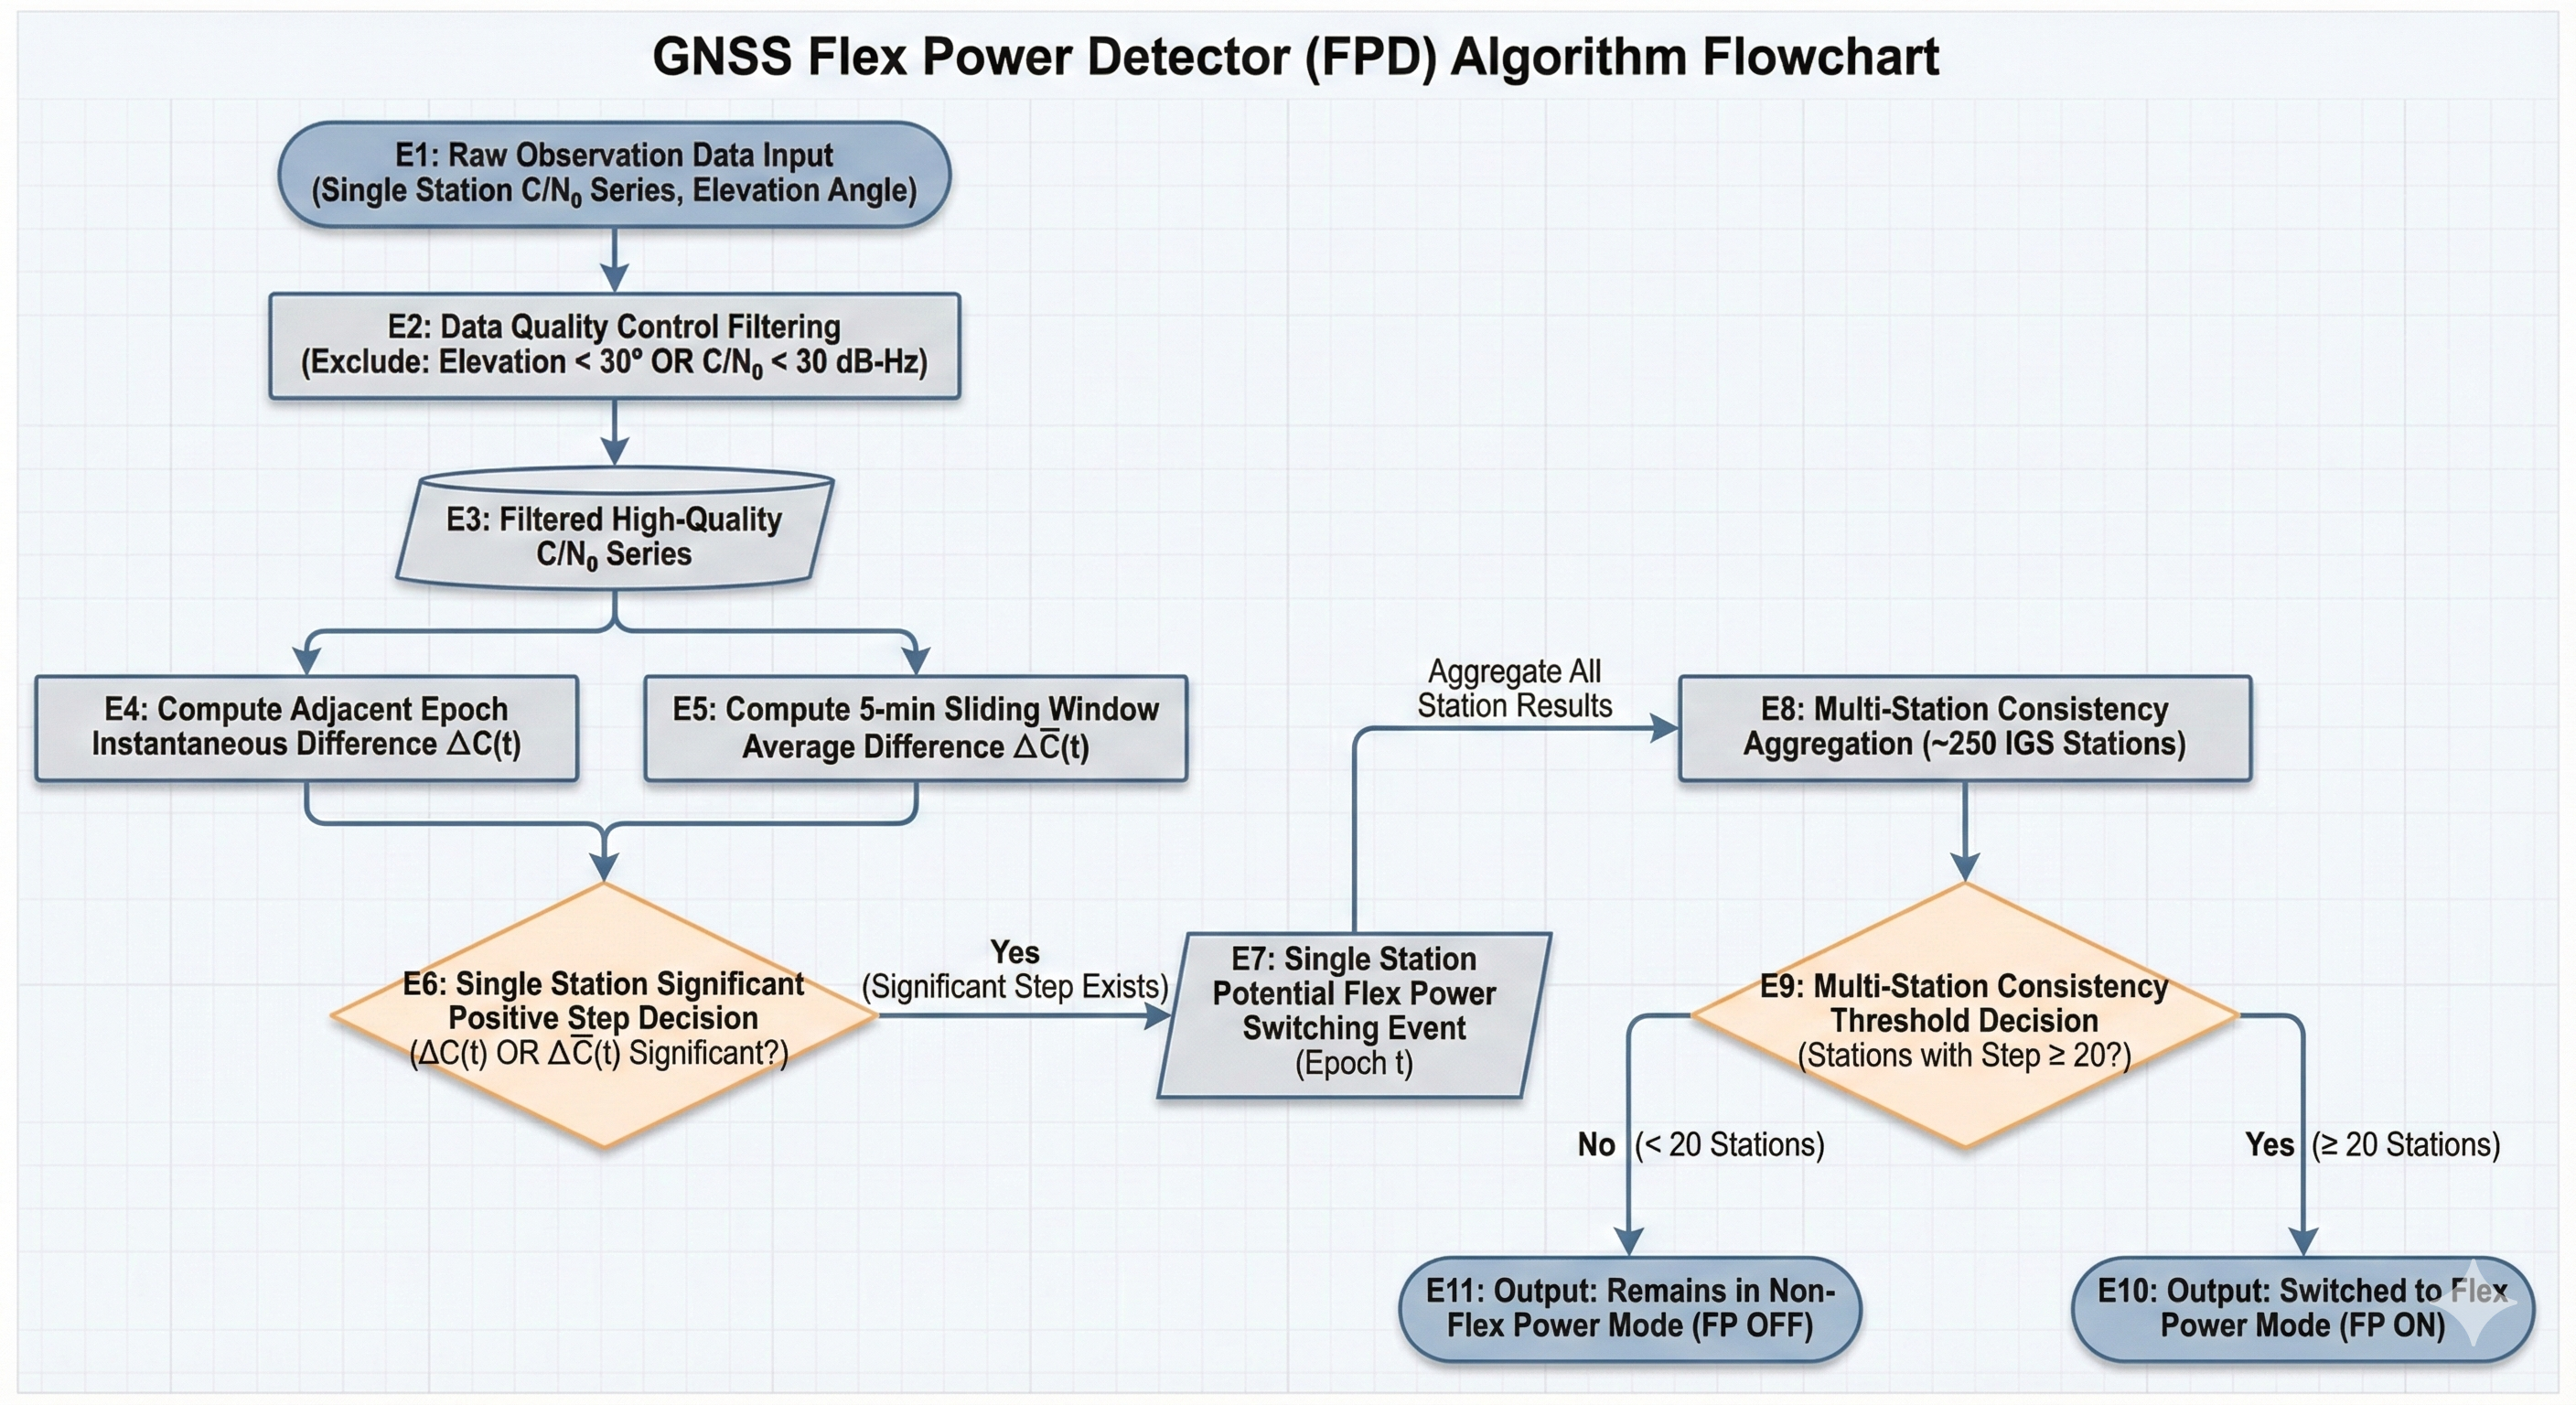
\includegraphics[width=0.8\linewidth]{figures/c3/fpd/flowchart.png}
    \bicaption{FPD算法整体流程图。其中FP表示Flex Power,即弹性功率}{Overall flowchart of the FPD algorithm, where FP denotes Flex Power.}
    \label{fig:fpd_flowchart}
\end{figure}

在具体实现中,如图\ref{fig:fpd_flowchart}所示,展示了FPD算法的完整流程。FPD 算法首先对原始观测数据进行质量控制。设某测站在历元 \(t\) 接收到的载噪比观测值为 \(C(t)\),FPD 仅保留满足高度角不小于 \(30^\circ\) 且
$ C(t) \ge 30~\mathrm{dB\!-\!Hz}$
的观测值,以减小低仰角与弱信号引入的噪声影响。
随后,对筛选后的 C/N0 序列计算相邻历元差分:
\begin{equation}
    \Delta C(t) = C(t) - C(t-1),
\end{equation}
用于捕获可能存在的瞬时阶跃变化。然而,考虑到部分弹性功率切换并非完全突变,而可能表现为短时间内的渐变特征,FPD 进一步引入滑动平均差分检测。具体而言,在当前历元 \(t\) 前后各取 \(5\) 分钟时间窗口(对应若干历元),分别计算窗口平均值:
\begin{equation}
    \bar{C}_{\text{pre}}(t), \qquad \bar{C}_{\text{post}}(t),
\end{equation}
并计算两者之差:
\begin{equation}
    \Delta \bar{C}(t) = \bar{C}_{\text{post}}(t) - \bar{C}_{\text{pre}}(t).
\end{equation}
该值能够有效反映缓变阶跃型的功率变化特征。

在单测站层面,若 \(\Delta C(t)\) 或 \(\Delta \bar{C}(t)\) 显示出显著的正向阶跃变化,则认为该测站在历元 \(t\) 检测到一次潜在的弹性功率切换事件。为避免由局部噪声或异常观测引起的误判,FPD 采用多测站一致性判决策略。具体的,在同一历元 \(t\),若在约 \(250\) 个 IGS 测站中,至少有 \(20\) 个测站同时检测到正向阶跃变化,则判定对应卫星在该历元切换至弹性功率(FP ON)模式;反之,则认为卫星处于非弹性功率(FP OFF)状态。通过结合单站阶跃检测与多站统计一致性判决,有效抑制了噪声和偶发异常的影响,实现了对 GNSS 卫星弹性功率切换的自动化、规模化检测。

基于上述原理,本文采用 FPD 算法对 BAIE 等 20 个 IGS 测站在 2020 年期间接收的 GPS 卫星S2W频点C/N0数据进行了弹性功率的事后处理检测。检测结果如表\ref{tab:mode_switch_s2w}所示,其中每个事件的检测结果为不同弹性功率模式之间的切换时间点,共14个切换点被成功检测出。而不同的切换点恰好对应了Esenbuuga等人对部分已知弹性功率模式的分类的时间边界点\cite{esenbuuga2023recent}。所有具有弹性功率功能的卫星S2W的平均抬升值列举在了表格的第4列,其中除了Mode4的平均抬升值在5.46dB,其余模式的平均抬升值都维持在9-10dB之间。模式转换列表示这一时间点从一个模式转换成了另一个模式,而None表示弹性功率功能的关闭。分析表格同时可以发现,弹性功率在GPS中的开启情况并不是罕见事件,而是处于长期开启情况,但是在不同模式之间存在频繁切换。根据人工核验载噪比时序的真值数据比较,发现FPD在2020年间的21个事件中,仅检测出17个事件,因此其召回率计算可得80.47\%,精确率为100\%,虚警率为0\%,F1-Score为89.47\%。

部分实验结果如图\ref{fig:fpd_result1}所示。其中,图\ref{fig:fpd_result2}给出了 2020 年 BAIE 测站接收的 G03 卫星 S2W 频点的原始 C/N0 时间序列及对应的 FPD 检测结果;根据esenbuuga等人对部分已知弹性功率模式的分类,此处对不同模式对应的时间区间采用不同颜色进行标注。图\ref{fig:fpd_result2}(b) 则展示了同一时间段内 BAIE 测站接收的 G05 卫星 S2W 频点的原始载噪比数据及其 FPD 检测结果,同样采用不同颜色对各类弹性功率模式进行覆盖。

\begin{table*}[htbp]
\centering
\bicaption{FPD 算法对 BAIE 等 20 个 IGS 测站在 2020 年期间接收的 GPS 卫星S2W频点载噪比数据进行了弹性功率的事后处理检测结果}{Post-processed flex power detection results of GPS S2W carrier-to-noise ratio data received by station BAIE and 20 other IGS stations in 2020 using the FPD algorithm}
\renewcommand{\arraystretch}{1.3}
\begin{tabularx}{\textwidth}{p{3cm} p{3cm} p{4cm} X}
\toprule
\textbf{切换点序号} & \textbf{日期} & \textbf{模式转换} & \textbf{卫星平均 S2W 抬升值} \\
\midrule

Mode 切换点 1  & 2020/2/14  & Mode1 $\rightarrow$ Mode4 & 5.46 dB-Hz \\

Mode 切换点 2  & 2020/5/4   & Mode4 $\rightarrow$ Mode5 & 9.43 dB-Hz \\

Mode 切换点 3  & 2020/5/5   & Mode5 $\rightarrow$ Mode6 & 9.79 dB-Hz \\

Mode 切换点 4  & 2020/5/9   & Mode6 $\rightarrow$ Mode5 & 9.43 dB-Hz \\

Mode 切换点 5  & 2020/6/14  & Mode5 $\rightarrow$ Mode7 & 9.36 dB-Hz \\

Mode 切换点 6  & 2020/6/20  & Mode7 $\rightarrow$ Mode5 & 9.43 dB-Hz \\

Mode 切换点 7  & 2020/6/23  & Mode5 $\rightarrow$ Mode7 & 9.36 dB-Hz \\

Mode 切换点 8  & 2020/7/3   & Mode7 $\rightarrow$ Mode5 & 9.43 dB-Hz \\

Mode 切换点 9  & 2020/8/3   & Mode5 $\rightarrow$ Mode7 & 9.36 dB-Hz \\

Mode 切换点 10 & 2020/8/22  & Mode7 $\rightarrow$ Mode8 & 9.95 dB-Hz \\

Mode 切换点 11 & 2020/9/13  & Mode8 $\rightarrow$ None  & 0 dB-Hz \\

Mode 切换点 12 & 2020/10/1  & None $\rightarrow$ Mode7  & 0 dB-Hz \\

Mode 切换点 13 & 2020/10/19 & Mode7 $\rightarrow$ Mode8 & 9.95 dB-Hz \\

Mode 切换点 14 & 2020/10/24 & Mode8 $\rightarrow$ Mode7 & 9.36 dB-Hz \\

Mode 切换点 15 & 2020/10/26 & Mode7 $\rightarrow$ Mode7 & 9.36 dB-Hz \\

Mode 切换点 16 & 2020/11/16 & Mode7 $\rightarrow$ Mode9 & 9.82 dB-Hz \\

Mode 切换点 17 & 2020/11/21 & Mode9 $\rightarrow$ Mode7 & 9.36 dB-Hz \\

\bottomrule
\end{tabularx}
\label{tab:mode_switch_s2w}
\end{table*}

当FPD检测异常值处于较低范围内时,说明没有发生窗口前后的值不连续性,表示没有弹性功率事件的发生。且由于硬件传输噪声原因,即使没有弹性功率功能变化,同样会有一定量的窗口差分值存在,表现为0均值附近波动的白噪声异常值。当FPD检测异常值处于较大值时,说明此时捕捉到了第二章所述的“阶跃提升”的特征,即卫星在测站可视范围内当日有弹性功率状态的切换。而不同大小的异常值则说明了不同弹性功率事件模式功率抬升值不同。

分析图\ref{fig:fpd_result1}与图\ref{fig:fpd_result2},可以直观发现,不同卫星的检测效果存在明显差异。相较于 G03 S2W,G05 S2W 的 FPD 检测结果整体表现较差:其异常值主要集中在 Mode6 与 Mode8 区间,仅在这些时间段被判定为弹性功率开启状态;而 G03 S2W 的检测结果则除 Mode9 未能成功识别外,其余弹性功率模式基本均得到了较为准确的探测。造成这种现象的原因是在第二章中提到过的:由于测站并不能对每一颗MEO卫星进行不间断的跟踪,每日仅能接收到部分信号,因此如果卫星发射端的弹性功率状态切换发生在测站可视范围外,就会导致“整体抬升”现象的发生。这一现象导致无法从非连续的时序中获得阶跃变化的特征被检测,从而无法实现弹性功率的正确识别。应对这一问题的方法则是使用足够多的测站(例如前文提及的250个测站)对同一颗卫星进行追踪,如果其中一定比例的测站检测出弹性功率事件,则判定为事件发生。

\begin{figure}
    \centering
    \includegraphics[width=1\linewidth]{figures/c3/fpd/result1.png}
    \bicaption{2020 年 BAIE 测站接收的 G03 卫星 S2W 频点的原始 C/N0 时间序列(上图)及对应的 FPD 检测结果(下图)}{Raw C/N0 time series of the G03 satellite at the S2W frequency received by the BAIE station in 2020 (upper panel) and the corresponding FPD detection results (lower panel)}
    \label{fig:fpd_result1}
\end{figure}

\begin{figure}
    \centering
    \includegraphics[width=1\linewidth]{figures/c3/fpd/result2.png}
    \bicaption{2020 年 BAIE 测站接收的 G05 卫星 S2W 频点的原始 C/N0 时间序列(上图)及对应的 FPD 检测结果(下图)}{Raw C/N0 time series of the G05 satellite at the S2W frequency received by the BAIE station in 2020 (upper panel) and the corresponding FPD detection results (lower panel)}
    \label{fig:fpd_result2}
\end{figure}

从图\ref{fig:fpd_result1}(a)中容易发现,S2W载噪比时序在Mode1和Mode4之间发生切换时刻有明显的不连续性,对应了图\ref{fig:fpd_result1}(b)中具有较大的异常值。相似的现象同样可以在Mode5和Mode6、Mode7和Mode8、Mode7和Mode9切换时刻发现。另一方面,在另外一些Mode的切换时刻,例如Mode4和Mode5之间切换时,却没有检测异常值的明显变化,因此理论上无法仅BAIE这一个测站上反应出不同Mode的切换情况。造成这种现象的原因是不同模式的弹性功率可能具有相同的载噪比抬升值,但是具有不同的物理开启区域,正如第二章的不同模式开启区域可视化图所示。如果要对不同弹性功率模式进行区分,则需要通过绘制多颗卫星的弹性功率开启时间轨迹以判断开启区域和开启中心是否存在模式差异。具体的实施方法会在后续AFPD-DTW方法实验结果分析部分展示。

此外,FPD 算法在应用过程中还需对载噪比数据进行高度角过滤,通常设置高度角截止值为 \(30^\circ\)。这是因为在低高度角条件下,C/N0 数据噪声水平较高,容易出现突变,这类突变恰好是 FPD 算法容易误判为弹性功率阶跃的特征,因此必须通过预处理加以抑制。然而,这种过滤策略也会导致大量观测数据被剔除,从而减少可用样本数量。对于弹性功率区域主要出现在较低高度角、或当日高高度角观测本身较少的情况,这种数据损失会显著增加检测难度。图\ref{fig:fpd_deAngle}展示了采用 \(30^\circ\) 高度角作为载噪比截止角后的数据分布情况,可以看出该阈值会过滤掉相当比例的有效观测信息。

\begin{figure}
    \centering
    \includegraphics[width=0.8\linewidth]{figures/c3/fpd/fpd_elangle.png}
    \bicaption{FPD高度角截止滤除数据示意图。绿色和红色的散点表示高于和低于30°高度角的载噪比数据。下方虚线表示高度角随时间的变化情况}{Schematic illustration of data filtering using an elevation angle cutoff in the FPD algorithm. Green and red scatter points indicate carrier-to-noise ratio data above and below an elevation angle of 30°, respectively. The dashed line in the lower panel represents the variation of elevation angle over time.}
    \label{fig:fpd_deAngle}
\end{figure}

在计算效率方面,大量实验表明 FPD 算法的整体耗时较长。在一台配置为 Intel(R) Core(TM) i7-9750H CPU @ 2.60\,GHz、内存 32.0\,GB 的计算机上,采用 C 语言实现的 FPD 算法对单一频点一整年的数据进行处理约需 20\,min,使用 Python 实现耗时约 21\,min,而 MATLAB 实现的处理时间则高达约 90\,min。考虑到实际应用中需要同时处理数百个 IGS 测站、多个卫星以及多频点数据,FPD 算法在整体计算量和时间消耗较大,这使其在实时弹性功率监测场景中的适用性受到明显限制。

\section{基于动态时间规划的差分检测方法(AFPD-DTW)}
虽然FPD检测算法通过多测站联合统计实现了弹性功率的自动化识别,但其核心机制仍存在两点显著局限。首先,FPD本质上是一种基于瞬时梯度特征的检测器,它高度依赖于观测序列中出现的显著阶跃信号。然而,实验表明,当卫星在测站视场外发生整体提升或处于低仰角区域时,这种阶跃特征往往无法被检测,导致召回率较低。其次,FPD需要使用大量测站来进行投票,无论是在后处理还是实时检测方面都对检测速度都不是最优方案。针对上述不足,本节提出了一种基于全序列模式匹配的新型检测方法——AFPD-DTW(Adaptive Flex Power Detector based on Dynamic Time Warping)。

\subsection{AFPD-DTW处理流程}
AFPD-DTW 的处理流程包括三个主要步骤,如图\ref{fig:afpd_4}所示。第一步是数据处理模块,它收集多站观测数据,包括观测文件、导航星历以及提供站坐标的 SINEX 文件。随后提取 C/N0 观测值,并与计算得到的卫星高度角进行结合。参考 FPD 方法\cite{esenbuuga2023recent}中的实际策略,为减轻多路径与噪声影响,剔除高度角低于 30° 的数据。

\begin{figure}
    \centering
    \includegraphics[width=1\linewidth]{figures/c3/afpd/图片4.png}
    \bicaption{AFPD-DTW流程图}{Pipeline of the AFPD-DTW.}
    \label{fig:afpd_4}
\end{figure}

第二步是将预处理后的数据输入 AFPD-DTW 检测模块。具体而言,当 AFPD-DTW 接收到新的数据时,若为事后处理,系统会首先检查当日序列是否完整;若不完整,则重置模型。而在实时检测中,则直接使用当前窗口的数据。随后流程会验证当前是否存在有效模型:若不存在,则将当前数据作为新模型,将该日标记为检测起始日,并等待下一批观测数据;若存在有效模型,则使用重叠序列计算 DTW 异常得分。当该得分超过由四分位距(IQR)方法确定的阈值时,即判定存在弹性功率事件;反之,则将当前数据纳入模型以进一步更新,从而增强模型的稳健性。

第三步是数据融合模块,用于对同一卫星的多站结果进行整合。具体而言,每颗卫星会对应多个 DTW 异常得分,这些得分通过加权投票方案进行融合,得到最终的异常得分。当该得分超过阈值时,即检测到弹性功率事件。为验证检测事件的空间一致性,还利用卫星地面轨迹检查激活区域及激活中心。最终输出内容包括检测到的弹性功率事件列表及对应的检测时间线。

\subsection{AFPD-DTW检测方法}
AFPD-DTW 的核心假设是:在非弹性功率条件下,GNSS 信号的 C/N0 时间序列呈现高度可重复的日周期模式。当目标日的序列模式与前几天存在显著偏离时,即表明发生了弹性功率变化。与基线建模方法相比,AFPD-DTW 使用前几天的稳定序列作为动态参考模型,并利用 DTW 计算当前序列与该模型之间的异常得分。

在事后处理模式下,设
\begin{equation}
    S_i = (s_{i,1}, s_{i,2}, \ldots, s_{i,T})
\end{equation}
表示需要检测的当天 C/N0 序列,其中 \(T\) 为当日观测历元数。该序列与前 \(N\) 天的平均序列比较:
\begin{equation}
    S_{\text{model}} = \frac{1}{N}\sum_{j=1}^{N} S_{i-j}.
\end{equation}
采用平均可平滑逐日波动,得到更稳健的参考序列。随后计算差分:
\begin{equation}
    \mathrm{diff}_S = S_i - S_{\text{model}}.
\end{equation}
若 \(\mathrm{diff}_S\) 超过阈值 \(\mathrm{thre}\),则判定为弹性功率事件。

然而,该直接差分方法虽然高效,但其对 C/N0 噪声非常敏感,易产生虚警。同时,由于序列间存在时间错位,即GPS 轨道重复周期为 11 h 58 min,而观测为 24 h 太阳日,导致逐日比较容易出错。

为解决上述问题,引入动态时间规整(Dynamic Time Warping, DTW)。DTW 通过动态对齐序列并计算最优路径距离来衡量相似性 \cite{berndt1994using}。给定模型序列 \(S_{\text{model}}\) 和目标序列 \(S_{\text{target}}\):
\begin{equation}
    S_{\text{model}} = (x_1, x_2, \ldots, x_N), \qquad\\
    S_{\text{target}} = (y_1, y_2, \ldots, y_M),
\end{equation}
其中 \(N\) 和 \(M\) 为两序列长度。定义局部距离函数:
\begin{equation}
    D(i,j) = d(x_i, y_j) = \lvert x_i - y_j \rvert.
\end{equation}
累积距离矩阵 \(C\) 通过下式递推得到:
\begin{equation}
    C(i,j) = D(i,j) + \min\left( C(i-1,j),\; C(i,j-1),\; C(i-1,j-1) \right),
\end{equation}
初始化为 \(C(1,1) = D(1,1)\)。最终 DTW 距离为
\begin{equation}
    \mathrm{DTW}(S_{\text{model}}, S_{\text{target}}) = C(N,M),
\end{equation}
作为异常度量,其值越小序列越相似,越大则可能存在弹性功率变化。检测规则为:
\begin{equation}
\begin{aligned}
\mathrm{DTW}_S > \mathrm{thre} &\Rightarrow \text{弹性功率事件}, \\
\mathrm{DTW}_S \le \mathrm{thre} &\Rightarrow \text{正常状态}.
\end{aligned}
\end{equation}


在实时检测中,设采样间隔为 \(\Delta t\),窗口长度为 \(W\)。定义当前窗口与模型窗口为:
\begin{equation}
\mathcal{W}_t = \{t-W+1, \ldots, t\},\qquad
S_i^t = \{ s_{i,\tau} \mid \tau \in \mathcal{W}_t \},\qquad
M_t = \{ m_\tau \mid \tau \in \mathcal{W}_t \}.
\end{equation}

其中 \(s_{i,\tau}\) 为第 \(i\) 天第 \(\tau\) 历元的 C/N0,\(m_\tau\) 为模型序列对齐至对应历元的值。

实时 DTW 使用 Sakoe–Chiba 带约束(半宽 \(r \le 3\)):
\begin{equation}
    \lvert p - q \rvert \le r.
\end{equation}
它限制时间偏移并将计算复杂度由 \(O(W^2)\) 降到 \(O(Wr)\)。

局部代价与带约束递推为:
\begin{equation}
    d(s_{i,\tau}, m_\kappa) = s_{i,\tau} - m_\kappa,
\end{equation}

\begin{equation}
C_t(p,q) = d(s_{i,t-W+p}, m_{t-W+q}) +
\min\left(
C_t(p-1,q),\;
C_t(p,q-1),\;
C_t(p-1,q-1)
\right),
\end{equation}
其中 \(p,q \in \{1,\ldots,W\}\) 且须满足 \(\lvert p-q \rvert \le r\),初始化为:
\begin{equation}
    C_t(1,1) = d(s_{i,t-W+1}, m_{t-W+1}).
\end{equation}
最优路径 \(P_t\) 的长度为 \(L(P_t)\),归一化 DTW 距离为:
\begin{equation}
    d_t = \frac{C_t(W,W)}{L(P_t)}.
\end{equation}
实时判决规则为:
\begin{equation}
\begin{cases}
d_t > \mathrm{thre}_{\mathrm{rt}}, & \text{弹性功率事件}, \\
d_t \le \mathrm{thre}_{\mathrm{rt}}, & \text{非事件}.
\end{cases}
\end{equation}

当不同日期处于相同的弹性功率状态时,DTW 值保持较低。如图\ref{fig:afpd_5}所示,可以观察到当两序列均为 FP OFF 状态时,残差小于 1,DTW 值为 116.92;当两序列均为 ON 且无阶跃偏移时,DTW = 76.91;当存在阶跃偏移时,尽管残差超过 5,DTW = 131.57 仍与前例接近,说明 DTW 能识别模式相似性且对时间偏移不敏感。

相比之下,当实际发生弹性功率变化时,DTW 值会显著升高。在图\ref{fig:afpd_5}(d)与图\ref{fig:afpd_5}(e)中,当 C/N0 数据出现阶跃式提升或整体提升时,DTW 值分别上升至 2368.88 和 2681.97,其量级比保持一致状态时高出一个数量级。

值得注意的是,DTW 同样能够有效处理中存在较强噪声的情况。在图\ref{fig:afpd_5}(f)中,尽管测试数据包含明显噪声,差分值最高达到 10,但 DTW 值仍保持在较低水平(286.04)。这种对噪声具有强鲁棒性的检测能力,使 DTW 方法能够同时适用于阶跃式提升和整体提升两类模式。

\begin{figure}
    \centering
    \includegraphics[width=1\linewidth]{figures/c3/afpd/图片5.png}
    \bicaption{在不同场景下,DTW 方法与差分方法的异常评分结果对比}{Anomaly scoring results of the DTW method and differential approach in different scenarios.}
    \label{fig:afpd_5}
\end{figure}

\subsection{阈值策略}
有效的阈值确定对于将 DTW 距离度量正确转化为弹性功率检测结果至关重要。阈值过小会导致误报,而阈值过大则会造成漏检。本文采用 IQR 方法,其自适应阈值特性在实际应用中效果良好。相比之下,静态阈值无法在不同卫星与站点之间通用,而机器学习方法则需要标注数据与频繁更新模型,因此均不适用于本场景。

首先从 DTW 序列 \( \mathrm{DTW}_S \) 中计算四分位数,即第 25 百分位数 \(Q_1\) 和第 75 百分位数 \(Q_3\)。随后计算 IQR:
\begin{equation}
    \mathrm{IQR} = Q_3 - Q_1.
\end{equation}

为了检测异常点,依据 IQR 定义上下阈值。通常使用系数 \(k\)(典型取值为 1.5):
\begin{equation}
\begin{aligned}
\text{Upper threshold} &= Q_3 + k \cdot \mathrm{IQR}, \\
\text{Lower threshold} &= Q_1 - k \cdot \mathrm{IQR}.
\end{aligned}
\end{equation}


对 DTW 序列中的每个数据点 \(x_i\) 与阈值进行比较,异常判断条件为:
\begin{equation}
x_i > Q_3 + k\cdot\mathrm{IQR}, \qquad\\
x_i < Q_1 - k\cdot\mathrm{IQR}.
\end{equation}
因此,最终的异常判定规则可写为:
\begin{equation}
\begin{cases}
\mathrm{DTW}_S > Q_3 + k\cdot\mathrm{IQR}, & \text{弹性功率事件}, \\
\mathrm{DTW}_S < Q_1 - k\cdot\mathrm{IQR}, & \text{弹性功率事件}, \\
Q_1 - k\cdot\mathrm{IQR} \le \mathrm{DTW}_S \le Q_3 + k\cdot\mathrm{IQR}, & \text{非弹性功率事件}.
\end{cases}
\end{equation}

\subsection{数据来源与预处理}
为了评估 AFPD-DTW 的性能,分别进行了事后处理检测与实时检测实验,使用的数据集如表\ref{tab:afpd_tab_1}所示。在事后处理检测中,使用了 2020--2025 年间来自 8 个 IGS 站点的每日 30 秒采样 S2W C/N0 数据,这些站点包括:AIRA、BIK0、CAS1、HAL1、HLFX、KAT1、SAVO 和 STFU。

\begin{table}[htbp]
\centering
\bicaption{AFPD-DTW实验的数据集}{Datasets of AFPD-DTW experiments.}
\label{tab:afpd_tab_1}

\renewcommand{\arraystretch}{1.2}
\begin{tabularx}{\textwidth}{
    p{1.5cm}   % 固定列 1
    p{2.0cm}     % 固定列 2
    p{1.5cm}         % 自动列 3
    X          % 自动列 4
    p{2.0cm}   % 固定列 5
}

\toprule
\textbf{实验类型} & \textbf{时间} &
\textbf{测站} &
\textbf{接收机-天线类型} &
\textbf{GNSS\&频段} \\
\midrule

\multirow{8}{*}{\textbf{后处理}}
& \multirow{8}{*}{\parbox{2cm}{\centering Jan 2020 - July 2025}}
& AIRA & TRIMBLE ALLOY / TRM59800.00 & \multirow{8}{*}{GPS--S2W} \\
& & BIK0 & SEPT POLARX5 / JAV\_RINGANT\_G3T & \\
& & CAS1 & TRIMBLE ALLOY / LEIAR25.R3 & \\
& & HAL1 & SEPT POLARX5 / JAVRINGANT\_DM & \\
& & HLFX & SEPT POLARX5 / TPSCR.G3 & \\
& & KAT1 & SEPT POLARX5 / LEIAR25.R3 & \\
& & SAVO & TRIMBLE NETR9 / TRM115000.00 & \\
& & STFU & JAVAD TRE\_G3TH / TRM57971.00 & \\
\midrule

\multirow{10}{*}{\textbf{实时处理}}
& \multirow{10}{*}{\parbox{2cm}{\centering June 1--7, 2024}}
& ABPO & SEPT POLARX5 / ASH701945G\_M & \multirow{10}{*}{GPS--S2W} \\
& & CUSV & JAVAD TRE\_3 DELTA / JAVRINGANT\_DM & \\
& & FAA1 & SEPT POLARX5 / LEIAR25.R4 & \\
& & KOKV & JAVAD TRE\_G3TH / ASH701945G\_M & \\
& & KOS1 & SEPT POLARX5E / LEIAR25.R3 & \\
& & KOUR & SEPT POLARX5TR / SEPCHOKE\_B3E6 & \\
& & MKEA & SEPT POLARX5 / JAVRINGANT\_DM & \\
& & NKLG & SEPT POLARX5 / TRM59800.00 & \\
& & NNOR & SEPT POLARX5TR / SEPCHOKE\_B3E6 & \\
& & OUS2 & SEPT POLARX5 / SEPCHOKE\_B3E6 & \\
\midrule

\textbf{多星座}
& Jan 2023 - July 2025
& 与后处理相同
& 与后处理相同
& BDS--S2I, S6I, S7I \\
\midrule
 
\textbf{多频段}
& Jan 2024 - July 2025
& 与后处理相同
& 与后处理相同
& GPS--S1C, S1W \\
\bottomrule
\end{tabularx}
\end{table}

随后,在实时检测实验中,选取了 2024 年 6 月 1 日至 2024 年 6 月 7 日期间来自 10 个 IGS 站点的数据:ABPO、CUSV、FAA1、KOKV、KOS1、KOUR、MKEA、NKLG、NNOR 和 OUS2。站点选择基于两个主要标准:  持续稳定的 C/N0 观测可用性与广泛的地理分布,以确保足够的空间覆盖与冗余。此外,通过 IGS 元数据对硬件一致性进行了验证。图\ref{fig:afpd_6}展示了参与这两项实验的站点分布,其中红色三角形与蓝色圆点分别代表用于事后处理与用于实时检测的站点。这些 30 秒数据均来自 CDDIS(\url{https://gdc.cddis.eosdis.nasa.gov/pub/gnss/data/daily})。

\begin{figure}
    \centering
    \includegraphics[width=0.5\linewidth]{figures/c3/afpd/图片6.png}
    \bicaption{用于 AFPD-DTW 检测中事后处理与实时处理实验的站点全球分布}{Global distribution of stations used for post-processing and real-time processing experiments in the AFPD-DTW detection.}
    \label{fig:afpd_6}
\end{figure}

在多星座与多频点验证方面,沿用事后处理实验中的同一批站点,对 2023 年 1 月至 2025 年 7 月期间的 BDS S2I、S6I 与 S7I 信号,以及 2024 年 7 月至 2025 年 7 月期间的 GPS S1C 与 S1W 信号进行了检测。

\subsection{基于AFPD-DTW方法的检测结果}
本节将通过事后处理、实时检测以及多星座/多频点检测实验对 AFPD-DTW 进行评估,并进一步与现有方法进行对比分析。

\subsubsection{后处理结果分析}
事后处理检测使用 2020--2025 年的全年数据进行验证。图\ref{fig:afpd_7}和图\ref{fig:afpd_8}展示了各站点的 S2W 信号 DTW 异常得分。在按天统计的异常得分中,数值越高表示发生弹性功率变化事件的可能性越大,不同颜色代表不同的卫星。图中可以清晰观察到某些日期多个卫星同时出现高异常得分的情况,特别是在 2021 年的弹性功率事件期间尤为明显。相比之下,2020 年的弹性功率事件更加集中,这与当年更复杂且频繁的弹性功率活动相对应。

\begin{figure}
    \centering
    \includegraphics[width=1\linewidth]{figures/c3/afpd/图片7.png}
    \bicaption{2020 年不同 GPS 卫星 S2W 信号的 DTW 异常得分时间序列。彩色圆点表示不同的 GPS 卫星。较高的 DTW 异常得分表示发生弹性功率变化事件的可能性更大}{Time series of DTW anomaly scores for S2W signals from different GPS satellites in 2020. Colored circular markers represent different GPS satellites. Higher DTW anomaly scores indicate a higher likelihood of flex power change events.}
    \label{fig:afpd_7}
\end{figure}

\begin{figure}
    \centering
    \includegraphics[width=1\linewidth]{figures/c3/afpd/图片8.png}
    \bicaption{2021 年不同 GPS 卫星 S2W 信号的 DTW 异常得分时间序列}{Time series of DTW anomaly scores for S2W signals from different GPS satellites in 2021.}
    \label{fig:afpd_8}
\end{figure}

需要注意的是,由于数据缺失,部分日期未显示异常得分,例如 CAS1 站在 2020 年 4 月至 6 月期间的缺测。通过多站点的验证发现:若具备高质量 C/N0 数据,即便使用极少量站点,也能够确定弹性功率激活日期。

为了识别具体的弹性功率事件日期,对 DTW 异常得分进行了异常检测。图\ref{fig:afpd_9}展示了基于动态 IQR 阈值方法的九组分类结果,用于区分弹性功率事件。由于弹性功率激活日期远少于非激活日期,IQR 分类器会将激活日期识别为异常点。对于分类表现欠佳的情况(如图\ref{fig:afpd_9}中 SAVO G01 与 G03),可通过多个站点与多个卫星的简单等权或加权投票策略有效避免误判。

表\ref{tab:afpd_tab_2}给出了 AFPD-DTW 事后处理算法在 2020 与 2021 年的弹性功率事件检测结果,这些结果与已有研究\cite{steigenberger2019flex,wu2024effects,meng2024real}报告的事件高度一致。表\ref{tab:afpd_tab_3}将 AFPD-DTW 的事后处理结果扩展至 2022 年 1 月至 2025 年 7 月的弹性功率事件,为后续相关研究提供了重要参考。此外,实验还识别出若干 FPD 未能检测到的弹性功率事件(以 * 标注),进一步验证了所提出算法的鲁棒性。

\begin{table*}[htbp]
\centering
\bicaption{2020--2021 年检测到的 GPS S2W 弹性功率变化事件(标注 * 的事件为以往方法未检测到)}{Detected GPS S2W flex power changes in 2020-2021. Events marked with * were missed by previous detection methods.}
\label{tab:afpd_tab_2}
% 如果你的模板支持 booktabs,建议添加 \usepackage{booktabs}
\begin{tabular}{cccccccc}
\hline % 若使用 booktabs 可改为 \toprule
\textbf{事件} & \textbf{日期} & \textbf{事件} & \textbf{日期} & \textbf{事件} & \textbf{日期} & \textbf{事件} & \textbf{日期} \\
\hline % 若使用 booktabs 可改为 \midrule

1  & 2020/2/14       & 12 & 2020/9/13        & 23 & 2021/1/16       & 34 & 2021/10/23 \\
2  & 2020/5/4        & 13 & \textbf{*2020/9/18} & 24 & 2021/3/5        & 35 & 2021/10/24 \\
3  & 2020/5/5        & 14 & \textbf{*2020/9/19} & 25 & 2021/3/6        & 36 & 2021/10/26 \\
4  & 2020/5/9        & 15 & 2020/10/1        & 26 & 2021/5/2        & 37 & 2021/10/27 \\
5  & 2020/6/14       & 16 & 2020/10/19       & 27 & 2021/5/17       & 38 & \textbf{*2021/11/3} \\
6  & 2020/6/20       & 17 & 2020/10/24       & 28 & 2021/5/31       & 39 & \textbf{*2021/11/4} \\
7  & 2020/6/23       & 18 & 2020/10/26       & 29 & 2021/6/5        & 40 & 2021/11/16 \\
8  & 2020/7/3        & 19 & 2020/11/5        & 30 & 2021/9/11       & 41 & 2021/11/17 \\
9  & \textbf{*2020/7/10} & 20 & 2020/11/16       & 31 & 2021/9/15       &    &  \\
10 & 2020/8/3        & 21 & 2020/11/21       & 32 & 2021/9/23       &    &  \\
11 & 2020/8/22       & 22 & 2021/1/12        & 33 & 2021/9/25       &    &  \\

\hline % 若使用 booktabs 可改为 \bottomrule
\end{tabular}
\end{table*}

\begin{table*}[htbp]
\centering
\bicaption{2022 年 1 月至 2025 年 7 月期间检测到的 GPS S2W 弹性功率变化事件}{Detected GPS S2W flex power changes from Jan 2022 to July 2025.}
\begin{tabularx}{\textwidth}{YYYYYYYY}
\hline
\textbf{Event} & \textbf{Date} & \textbf{Event} & \textbf{Date} &
\textbf{Event} & \textbf{Date} & \textbf{Event} & \textbf{Date} \\
\hline

1 & 2022/5/24 & 30 & 2023/6/22 & 59 & 2023/11/6 & 88 & 2024/2/17 \\
2 & 2022/5/25 & 31 & 2023/6/23 & 60 & 2023/11/7 & 89 & 2024/3/5 \\
3 & 2022/6/13 & 32 & 2023/6/24 & 61 & 2023/11/9 & 90 & 2024/4/29 \\
4 & 2022/6/18 & 33 & 2023/6/26 & 62 & 2023/11/10 & 91 & 2024/4/30 \\
5 & 2022/7/11 & 34 & 2023/6/27 & 63 & 2023/12/4 & 92 & 2024/5/10 \\
6 & 2022/7/12 & 35 & 2023/6/29 & 64 & 2023/12/8 & 93 & 2024/5/11 \\
7 & 2022/7/16 & 36 & 2023/7/22 & 65 & 2023/12/11 & 94 & 2024/5/26 \\
8 & 2022/8/18 & 37 & 2023/7/29 & 66 & 2023/12/12 & 95 & 2024/5/27 \\
9 & 2022/8/19 & 38 & 2023/8/22 & 67 & 2023/12/14 & 96 & 2024/6/4 \\
10 & 2022/8/20 & 39 & 2023/8/23 & 68 & 2024/1/4 & 97 & 2024/6/7 \\
11 & 2022/8/21 & 40 & 2023/8/24 & 69 & 2024/1/19 & 98 & 2024/6/8 \\
12 & 2022/8/22 & 41 & 2023/8/25 & 70 & 2024/1/20 & 99 & 2024/6/15 \\
13 & 2022/8/23 & 42 & 2023/8/26 & 71 & 2024/1/20 & 100 & 2024/6/26 \\
14 & 2022/8/24 & 43 & 2023/8/27 & 72 & 2024/1/21 & 101 & 2024/6/27 \\
15 & 2022/9/6 & 44 & 2023/8/28 & 73 & 2024/1/22 & 102 & 2024/7/25 \\
16 & 2022/9/7 & 45 & 2023/8/29 & 74 & 2024/1/23 & 103 & 2024/7/26 \\
17 & 2022/9/10 & 46 & 2023/9/21 & 75 & 2024/1/24 & 104 & 2025/3/31 \\
18 & 2022/9/18 & 47 & 2023/9/22 & 76 & 2024/1/25 & 105 & 2025/4/4 \\
19 & 2022/9/26 & 48 & 2023/9/23 & 77 & 2024/1/26 & 106 & 2025/4/5 \\
20 & 2022/10/3 & 49 & 2023/9/24 & 78 & 2024/1/30 & 107 & 2025/4/12 \\
21 & 2022/10/6 & 50 & 2023/10/3 & 79 & 2024/1/31 & 108 & 2025/4/14 \\
22 & 2022/12/5 & 51 & 2023/10/4 & 80 & 2024/2/1 & 109 & 2025/4/19 \\
23 & 2022/12/10 & 52 & 2023/10/6 & 81 & 2024/2/2 & 110 & 2025/4/28 \\
24 & 2023/4/24 & 53 & 2023/10/7 & 82 & 2024/2/5 & 111 & 2025/4/29 \\
25 & 2023/4/25 & 54 & 2023/10/24 & 83 & 2024/2/6 & 112 & 2025/5/1 \\
26 & 2023/4/28 & 55 & 2023/10/25 & 84 & 2024/2/9 & 113 & 2025/5/8 \\
27 & 2023/4/29 & 56 & 2023/10/26 & 85 & 2024/2/10 & 114 & 2025/5/9 \\
28 & 2023/5/1 & 57 & 2023/11/1 & 86 & 2024/2/14 & 115 & 2025/5/13 \\
29 & 2023/5/16 & 58 & 2023/11/2 & 87 & 2024/2/15 &     &        \\

\hline
\end{tabularx}
\label{tab:afpd_tab_3}
\end{table*}

图\ref{fig:afpd_10}展示了三例 AFPD-DTW 成功检测而 FPD 未检测到的 2020--2021 年多站点 S2W C/N0 时间序列。其中不同颜色的点代表不同站点的观测,红色与绿色阴影线分别表示弹性功率的激活与关闭区间,并附有时间戳。

\begin{figure}
    \centering
    \includegraphics[width=1\linewidth]{figures/c3/afpd/图片9.png}
    \bicaption{基于动态 IQR 阈值的方法用于区分多站点–多卫星组合的 S2W 信号中的弹性功率事件(红色)与非事件(蓝色)}{Dynamic IQR threshold method applied to distinguish flex power events (red) and non-events (blue) in S2W signals across various station-satellite combinations.}
    \label{fig:afpd_9}
\end{figure}

例如,2020 年 7 月 8 日与 9 日,G05 的弹性功率分别在 1:24 关闭、11:25 激活,而在 7 月 10 日,这两个时刻变为 0:22 与 13:15,显示出模式转换。2020 年 9 月 18 日,弹性功率切换到全球覆盖模式,并于 9 月 19 日关闭。类似地,2021 年 11 月 3 日,激活/关闭时间由 00:00/12:00 突然变为 00:00/3:01,表明发生了另一次模式变化。这些模式转换均被 AFPD-DTW 成功检出,而 FPD 未能识别,进一步凸显了本方法的有效性。

\subsubsection{实时结果分析}
为了确保实时检测中对全天信号的完整覆盖,使用了 10 个站点在 2024 年 6 月 1--7 日期间的观测数据。图\ref{fig:afpd_11}给出了 AFPD-DTW 的实时检测结果,其中蓝色、绿色、红色和橙色分别表示 TP、TN、FP 和 FN。表\ref{tab:afpd_tab_4}的性能分析显示,AFPD-DTW 在实时检测中具有极高的可靠性。对所有 PRN 而言,TPR 均超过 99.6\%,其中 G15 的检测率最高,达到 99.93\%。FPR 极低,G01、G05、G06、G25 和 G31 的假阳性率为零。整体准确度(Accuracy)始终保持在 99.74\% 至 99.97\% 之间。Precision 表现尤为优秀,多颗卫星达到 100\%,最低 Precision 也超过 99.95\%。总体而言,AFPD-DTW 的平均 TPR 为 99.86\%,FPR 为 0.053\%,Accuracy 为 99.88\%,Precision 为 99.98\%,充分展示了其在实时弹性功率检测中的卓越性能。

模式 1 具有区域覆盖特征,覆盖范围为 30°W 至 150°E,但未呈现明显的激活中心(见图\ref{fig:afpd_12})。相比之下,模式 2 提供全球覆盖(见图\ref{fig:afpd_13})。

\begin{figure}
    \centering
    \includegraphics[width=1\linewidth]{figures/c3/afpd/图片10.png}
    \bicaption{2020–2021 年期间多站 S2W C/N0 时间序列中由 FPD 漏检的三次弹性功率模式转换}{Multi-station S2W C/N0 time series depicting three flex power mode transitions overlooked by FPD during 2020-2021.}
    \label{fig:afpd_10}
\end{figure}

与此同时,图\ref{fig:afpd_11}还揭示了检测期间弹性功率模式随时间的显著变化。在观测时段内,共检测到两种模式。模式 1 出现在 6 月 1--3 日及 6 月 7 日的部分时间段内;而模式 2 则在 6 月 4--6 日全天处于激活状态。表\ref{tab:afpd_tab_5}总结了这两种模式的开始与结束时间戳,其差异十分明显。

\begin{figure}
    \centering
    \includegraphics[width=0.5\linewidth]{figures/c3/afpd/图片11.png}
    \bicaption{2024 年 6 月 1 日至 8 日期间 GPS 卫星的 AFPD-DTW 实时检测结果}{Results of AFPD-DTW real-time detection for GPS satellites from June 1 to 8, 2024.}
    \label{fig:afpd_11}
\end{figure}

\begin{table*}[htbp]
\centering
\bicaption{2024 年 6 月 1--7 日期间基于 S2W 信号的 IIR-M 与 IIF 卫星实时检测性能(\%)}{Real-time detection performance (\%) on IIR-M and IIF satellites in the S2W signal from June 1–7, 2024.}
\begin{tabular}{lcccc @{\quad} lcccc}
\hline
\textbf{PRN} & \textbf{TPR} & \textbf{FPR} & \textbf{Accuracy} & \textbf{Precision} &
\textbf{PRN} & \textbf{TPR} & \textbf{FPR} & \textbf{Accuracy} & \textbf{Precision} \\
\hline

\textbf{G01} & 99.89 & 0    & 99.92 & 100    &
\textbf{G17} & 99.79 & 0.08 & 99.82 & 99.97 \\

\textbf{G03} & 99.85 & 0.09 & 99.87 & 99.97 &
\textbf{G24} & 99.92 & 0.04 & 99.93 & 99.99 \\

\textbf{G05} & 99.92 & 0    & 99.94 & 100    &
\textbf{G25} & 99.90 & 0    & 99.93 & 100    \\

\textbf{G06} & 99.77 & 0    & 99.83 & 100    &
\textbf{G26} & 99.92 & 0.04 & 99.93 & 99.99 \\

\textbf{G07} & 99.95 & 0.10 & 99.94 & 99.97 &
\textbf{G27} & 99.92 & 0.06 & 99.92 & 99.98 \\

\textbf{G08} & 99.79 & 0.07 & 99.82 & 99.98 &
\textbf{G29} & 99.87 & 0.12 & 99.87 & 99.95 \\

\textbf{G09} & 99.93 & 0.09 & 99.93 & 99.97 &
\textbf{G30} & 99.77 & 0.08 & 99.81 & 99.97 \\

\textbf{G10} & 99.66 & 0.04 & 99.74 & 99.99 &
\textbf{G31} & 99.77 & 0    & 99.83 & 100 \\

\textbf{G12} & 99.98 & 0.07 & 99.97 & 99.97 &
\textbf{G32} & 99.77 & 0.12 & 99.80 & 99.96 \\

\textbf{G15} & 99.93 & 0.02 & 99.95 & 99.99 &
\textbf{Ave} & 99.86 & 0.05 & 99.88 & 99.98 \\
\hline
\end{tabular}
\label{tab:afpd_tab_4}
\end{table*}

\begin{table}[htbp]
\centering
\bicaption{2024 年 6 月 2 日 GPS S2W 弹性功率激活时间段}{Activation periods of GPS flex power in S2W on June 2, 2024.}
\label{tab:afpd_tab_5}
\begin{tabularx}{\textwidth}{YYYYYYYY}
\hline
\textbf{PRN} & \textbf{Block} & \textbf{Start} & \textbf{End} & 
\textbf{PRN} & \textbf{Block} & \textbf{Start} & \textbf{End} \\
\hline

\textbf{G01} & IIF   & 07:12:00 & 18:59:30 & \textbf{G15} & IIR-M & 00:00:00 & 11:23:30 \\
\textbf{G03} & IIF   & 00:00:00 & 02:00:30 &              &       & 23:24:00 & 23:59:30 \\
             &       & 14:00:30 & 23:59:30 & \textbf{G17} & IIR-M & 00:00:00 & 06:36:00 \\
\textbf{G05} & IIR-M & 00:00:00 & 09:35:30 &              &       & 18:36:00 & 23:59:30 \\
             &       & 21:36:00 & 23:59:30 & \textbf{G24} & IIF   & 01:00:30 & 13:00:00 \\
\textbf{G06} & IIF   & 00:00:00 & 05:48:00 & \textbf{G25} & IIF   & 03:24:30 & 15:24:00 \\
             &       & 17:49:00 & 23:59:30 & \textbf{G26} & IIF   & 07:24:30 & 19:24:00 \\
\textbf{G07} & IIR-M & 00:00:00 & 03:24:00 & \textbf{G27} & IIF   & 09:48:30 & 21:48:00 \\
             &       & 15:24:00 & 23:59:30 & \textbf{G29} & IIR-M & 01:48:00 & 13:36:00 \\
\textbf{G08} & IIF   & 11:13:00 & 23:59:30 & \textbf{G30} & IIF   & 00:00:00 & 04:48:30 \\
\textbf{G09} & IIF   & 00:00:00 & 02:24:00 &              &       & 16:49:00 & 23:59:30 \\
             &       & 14:24:30 & 23:59:30 & \textbf{G31} & IIR-M & 07:24:00 & 19:23:30 \\
\textbf{G10} & IIF   & 06:24:30 & 18:24:00 & \textbf{G32} & IIF   & 07:12:30 & 19:12:00 \\
\textbf{G12} & IIR-M & 00:00:00 & 11:48:00 &              &       &          &          \\
             &       & 23:48:30 & 23:59:30 &              &       &          &          \\

\hline
\end{tabularx}
\end{table}

\begin{figure}
    \centering
    \includegraphics[width=0.85\linewidth]{figures/c3/afpd/图片12.png}
    \bicaption{2024 年 6 月 2 日期间具有弹性功率激活的 GPS 卫星轨迹}{GPS satellite trajectory with flex power activation on June 2, 2024.}
    \label{fig:afpd_12}
\end{figure}

\begin{figure}
    \centering
    \includegraphics[width=0.85\linewidth]{figures/c3/afpd/图片13.png}
    \bicaption{2024 年 6 月 4 日期间具有弹性功率激活的 GPS 卫星轨迹}{GPS satellite trajectories with flex power activation on June 4, 2024.}
    \label{fig:afpd_13}
\end{figure}

\subsubsection{多星座与多频段检测}
为了评估 AFPD-DTW 在多星座与多频点场景中的适用性,采用了表\ref{tab:afpd_tab_1}中事后处理实验使用的同一组站点。对于BDS,对 2023 年 1 月至 2025 年 7 月期间的 S2I、S6I 和 S7I 信号进行了分析;对于 GPS,则分析了 2024 年 1 月至 2025 年 7 月期间的 S1C 与 S1W 信号。

\begin{table*}[htbp]
\centering
\bicaption{多星座与多频点弹性功率事件检测结果:BDS(2023 年 1 月--2025 年 7 月)与 GPS(2024 年 1 月--2025 年 7 月)}{Multi-constellation and multi-frequency flex-power events detected from BDS (January 2023 – July 2025) and GPS (January 2024 – July 2025).}
\label{tab:afpd_tab_6}
\begin{tabular}{lcccc}
\hline
\textbf{星座} & \textbf{事件编号} & \textbf{日期} & \textbf{频点} & \textbf{PRNs} \\
\hline

\multirow{10}{*}{\textbf{BDS}}
& 1 & 2023/9/27 & \multirow{10}{*}{S6I}
& IGSO: C06, C07, C08, C09, C10, C13, C16 \\

& 2 & 2023/9/30 &  
& IGSO: C07, C09, C10, C13, C16 \\

& 3 & 2024/9/23 & 
& MEO: C11, C12, C14 \\

& 4 & 2024/9/30 &
& IGSO: C07, C08, C09, C10, C13, C16; MEO: C11, C12 \\

& 5 & 2024/10/29 &
& IGSO: C07, C08, C09, C10, C13, C16 \\

& 6 & 2024/10/30 &
& MEO: C11, C12 \\

& 7 & 2024/11/9 &
& IGSO: C07, C09, C10, C16 \\

& 8 & 2024/11/12 &
&  \\

& 9 & 2025/4/19 &
& IGSO: C07, C08, C09, C10, C13, C16 \\

& 10 & 2025/4/23 &
& IGSO: C07, C08, C09, C10, C13, C16 \\
\hline

\multirow{14}{*}{\textbf{GPS}}
& 1 & 2024/7/25 & S1W &  \\

& 2 & 2024/7/26 &
& G01, G03, G05, G06, G07, G08, G09, G10, G12, G15, \\
&   &           &
& G17, G24, G25, G26, G27, G29, G30, G31, G32 \\

& 3 & 2025/3/31 &
&  \\

& 4 & 2025/4/4 &
&  \\

& 5 & 2025/4/5 &
&  \\

& 6 & 2025/4/12 &
&  \\

& 7 & 2025/4/14 &
&  \\

& 8 & 2025/4/19 &
& G03, G05, G06, G07, G08, G09, G10, G12, G15, G17, \\
&   &           &
& G24, G25, G26, G27, G29, G30, G31, G32 \\

& 9 & 2025/4/28 &
&  \\

& 10 & 2025/4/29 &
&  \\

& 11 & 2025/5/1 &
&  \\

& 12 & 2025/5/8 &
&  \\

& 13 & 2025/5/9 &
&  \\

& 14 & 2025/5/13 &
&  \\

\hline
\end{tabular}

\end{table*}

结果汇总于表\ref{tab:afpd_tab_6}。未在 BDS 的 S2I 与 S7I 信号,以及 GPS 的 S1C 信号中检测到弹性功率事件。对于 GPS S1W,所有检测到的事件均与 S2W 信号上观测到的事件完全一致。此外,观察到自 2025 年之后,卫星 G01 不再参与任何事件。经官方记录验证得知,2025 年 1 月 22 日,G01 从 SVN63(Block IIR-M)切换至 SVN80(Block III)\cite{IS},进一步说明目前具备弹性功率能力的主要为 GPS Block IIR-M 与 IIF 卫星。

在 BDS S6I 信号上共检测到十次弹性功率事件,且全部发生在 BDS-2 卫星上。进一步分析表明,具有弹性功率功能的北斗卫星均为 IGSO 或 MEO 卫星,而 GEO 卫星未受到影响。

通过卫星地面轨迹进行验证,以确认弹性功率激活的实际存在。如图\ref{fig:apfd_14}所示,展示了两个北斗弹性功率事件的示例。区别在于:2023 年的事件同时影响了 IGSO 与 MEO 卫星,而 2024 年的事件仅涉及 IGSO 卫星。两种情况下,深色阴影区域均对应弹性功率的影响范围。

\begin{figure}
    \centering
    \includegraphics[width=0.85\linewidth]{figures/c3/afpd/图片14.png}
    \bicaption{2024 年 9 月 23 日和 2023 年 9 月 27 日 BDS 卫星在 S6I 信号上触发弹性功率时的轨迹}{BDS satellite trajectories with flex power activation on 2024-09-23 and 2023-09-27 on S6I.}
    \label{fig:apfd_14}
\end{figure}

值得注意的是,与 GPS S2W 信号不同,BDS S6I 信号在激活区域外表现出增强,而在区域内却表现为关闭状态。这可能表明在这两次北斗事件中,S6I 频段的发射功率被重新分配至其他频段,但这些频段的数据并未可用。

\subsubsection{比较与分析}
AFPD-DTW 方法与以往方法的综合性能对比见表\ref{tab:afpd_tab_7}和\ref{tab:afpd_tab_8}。通过 C/N0 时间序列与卫星轨迹对多星座、多频点的弹性功率状态进行了人工核查,AFPD-DTW 在事后处理检测中取得了 99.94\% 的准确率(Accuracy)。在实时检测中,AFPD-DTW 的 TPR 达到 99.87\%,并在仅使用 10 个站点的情况下保持了 99.89\% 的检测精度与 99.98\% 的精确率(Precision)。若进一步结合更多站点数据,这些指标仍有提升空间。

\begin{table*}[htbp]
\centering
\bicaption{各类弹性功率检测算法性能对比\cite{yang2022real,esenbuuga2023recent,meng2024real}}{Comparison of detection performance(\%) of various flex power detection algorithms\cite{yang2022real,esenbuuga2023recent,meng2024real}}
\begin{tabular}{lcccc}
\hline
\textbf{方法} & \textbf{年份} & \textbf{应用场景} & \textbf{数据需求} & \textbf{星座} \\
\hline

FPD & 2023 & 事后处理 & 需要超过 200 个站点数据 & GPS \\

RF-based & 2022 & 实时检测 & 每个站点均需训练数据集 & GPS \\

Baseline-modeling & 2024 & 实时检测 & 需要含已知弹性功率状态的历史数据 & GPS \\

AFPD-DTW & 2025 & 事后处理 / 实时检测 & 仅需 8--10 个站点;无历史数据需求 & GPS / BDS \\
\hline
\end{tabular}
\label{tab:afpd_tab_7}
\end{table*}

\begin{table*}[htbp]
\centering
\bicaption{AFPD-DTW 在多星座与多频点场景下的整体检测性能}{Overall detection performance of AFPD-DTW across multi-constellation and multi-frequency scenarios}
\begin{tabular}{lcccccc}
\hline
\textbf{场景} & \textbf{星座/频率} & \textbf{时间} 
& \textbf{Acc (\%)} & \textbf{Prec (\%)} & \textbf{TPR (\%)} & \textbf{FPR (\%)} \\
\hline

\multirow{3}{*}{\textbf{后处理}} 
& GPS S2W & Jan 2020--July 2025 & 99.91 & 99.36 & 99.36 & 0.05 \\
& BDS S6I & Jan 2023--July 2025 & 100 & 100 & 100 & 0 \\
& Total   &  & 99.94 & 99.4 & 99.4 & 0.03 \\

\hline

\multirow{3}{*}{\textbf{实时}} 
& GPS S2W & June 1--7, 2024 & 99.88 & 99.98 & 99.86 & 0.05 \\
& BDS S6I & Sept 23--30, 2024 & 99.91 & 99.99 & 99.88 & 0.04 \\
& Total   &  & 99.89 & 99.98 & 99.87 & 0.04 \\

\hline
\end{tabular}
\label{tab:afpd_tab_8}
\end{table*}

在数据需求方面,AFPD-DTW 不依赖历史数据,仅需 8--10 个站点即可运行,因此能够在多星座、多频点环境中实现快速、简化的部署。相比之下,FPD 需要超过 200 个站点,而基于随机森林的方法需要大量标注训练数据;基于模型的方法则依赖大规模先验数据集和特定硬件配置。

在检测效率方面,由于 AFPD-DTW 仅使用少量站点数据,相比 FPD 实现了约 20 倍的加速。这种大幅度的速度提升使得快速事后处理与实时检测成为可能,尤其是在站网规模不断扩大、卫星星座数量持续增长的背景下,其重要性更加显著。

总之,AFPD-DTW 通过利用卫星日周期 C/N0 差分特性,并采用 DTW 校正周期不匹配问题,实现了高效且可靠的弹性功率检测。在实时与事后处理两种模式下,它在保持高精度的同时显著提升了检测速度,且对数据需求极低,无需任何预训练的基线模型。


\section{DLFPD 网络架构设计}
尽管 AFPD-DTW 在处理时间错位和噪声方面表现出色,但其本质上属于一种相对检测策略。它依赖于将当前观测值与历史基准进行差分比较。这种机制存在两个固有的局限性。首先,它对初始状态敏感,需要人为确认基准日处于非弹性功率状态;其次,当弹性功率事件基准模型不稳定时,差分方法可能失效,从而难以判断当前的绝对功率状态。

为了克服上述缺陷,本节提出一种基于深度学习的端到端检测框架(DLFPD, Deep Leaening-Based Flex Power Detector)。该方法的核心目标是构建一个具有高泛化能力的通用模型,旨在通过单一模型实现对不同测站、不同卫星对的实时状态判读,而无需针对特定链路进行独立建模。本质上,该方法将弹性功率检测建模为一个多变量时间序列分类问题,即以归一化的信号强度序列及空间几何特征为输入,通过混合神经网络架构提取深层特征,最终输出当前时刻发生弹性功率事件的绝对概率。

\subsection{DLFPD方法}
图\ref{fig:c3_dl_strcut}展示了用于弹性功率检测的DLFPD架构。

\begin{figure}[htbp]
\centering
\includegraphics[width=1\linewidth]{figures/c3/DLFPD/struct2.png}
\bicaption{DLFPD架构}{Structure of DLFPD.}
\label{fig:c3_dl_strcut}
\end{figure}

\subsubsection{数据预处理与特征工程}
深度学习模型的性能高度依赖于输入数据的质量与表征形式。原始数据包括带有时间戳的 GNSS 信号日志、测站坐标、卫星位置以及不同信号分量的C/N0。

弹性功率 检测的关键物理量为主信号($S_1$)、副信号($S_2$)的 C/N0 值及其差值($\Delta_{\text{diff}} = S_2 - S_1$)。由于不同接收机、不同仰角下的基准噪声水平存在显著差异,直接使用原始分贝值会导致模型难以收敛。因此,采用 Z-Score 标准化处理:
\begin{equation}
    x_{\text{norm}} = \frac{x - \mu_{\text{global}}}{\sigma_{\text{global}}},
\end{equation}
其中,$\mu_{\text{global}}$ 和 $\sigma_{\text{global}}$ 是在训练集上预先计算的全局均值和标准差。

为了捕捉信号的瞬态特征与动态趋势,构建了复合输入向量。其中的当前状态向量为时间点 $t$ 的 $S_1$、$S_2$ 和 $\Delta_{\text{diff}}$ 的瞬时归一化值。其中的时序序列窗口向量则是构建长度为 $W$ 的滑动窗口序列 $X_{seq} = [x_{t-W+1}, \dots, x_t]$。这使模型能够观察信号在短时间内的变化模式,从而区分噪声引起的波动与功率阶跃。

GNSS 信号强度受多径效应和卫星机动影响显著。为了解耦这些环境因素,设计了显式上下文嵌入。第一种周期性时间编码为了保持时间的连续性(例如 23:59 与 00:01 的邻近性),此处将时间分量 $v$(如小时、DOY)分解为正弦与余弦特征:
\begin{equation}
    v_{\text{cyc}} = \left[ \sin\left(\frac{2\pi v}{P}\right), \cos\left(\frac{2\pi v}{P}\right) \right].
\end{equation}
第二种是几何特征嵌入,即卫星的高度角 $\theta_{el}$ 和方位角 $\theta_{az}$ 通过三角函数变换映射为连续特征,以辅助模型识别低高度角下的自然多径衰减。

第三种卫星身份嵌入表示了不同批次(Block)的卫星可能具有不同的功率特性。此处使用可学习的嵌入层将离散的卫星 PRN 编号映射为密集向量 $E_{\text{sat}} \in \mathbb{R}^{32}$,使模型能够自适应地学习特定卫星的硬件偏差。

\subsubsection{混合神经网络架构}
为了兼顾局部特征提取与全局依赖建模,本文提出了一个混合 CNN-Transformer 网络架构。该架构包含双通道特征提取模块与多模态融合模块。

针对输入的时序信号 $X_{seq}$,设计了双路并行处理分支。第一个通道为多尺度 CNN 分支,用于捕捉局部突变。采用一维卷积神经网络(1D-CNN),堆叠三个卷积块,卷积核尺寸依次递增 ($k=[3, 5, 7]$)。每个卷积块包含卷积层、批归一化(Batch Normalization, BN)、ReLU 激活函数和 Dropout 层。第二路通道为Transformer 分支,用于捕捉长程依赖。引入 Transformer 编码器,利用多头自注意力机制(Multi-Head Self-Attention)分析窗口内的全局上下文关联\cite{vaswani2017attention}:
\begin{equation}
    \text{Attention}(Q, K, V) = \text{softmax}\left(\frac{QK^T}{\sqrt{d_k}}\right)V.
\end{equation}
这使得模型在判断当前时刻状态时,能够有效利用窗口早期的信号趋势作为参考。

模型的最终判决基于多源信息的整合,通过将 CNN 提取的局部特征向量、Transformer 提取的全局特征向量、卫星嵌入 $E_{\text{sat}}$ 以及时空编码特征拼接为统一的特征向量 $F_{\text{fused}}$。该向量随即通过一个包含层归一化(LayerNorm)和 ReLU 的多层感知机(Multi Layer Perceptron, MLP)融合模块,以建模不同模态间的非线性交互。最后,通过全连接层与 Sigmoid 激活函数,输出当前历元发生弹性功率事件的概率 $P(y=1|x)$。

\subsubsection{损失函数与模型训练}
由于弹性功率事件在长期观测中属于稀疏事件,正负样本比例极不平衡。若使用标准交叉熵损失,模型倾向于预测出无事件以获得较高的统计精度\cite{mao2023cross}。为此,设计了复合损失函数 $\mathcal{L}_{\text{total}}$。

采用 Focal Loss \cite{lin2017focal}降低存在大量正常观测数据的简单负样本情况下在梯度更新中的权重,迫使模型专注于难以分类的样本:
\begin{equation}
    \mathcal{L}_{\text{Focal}}(p_t) = -\alpha (1-p_t)^\gamma \log(p_t),
\end{equation}
其中 $p_t$ 为模型对真实类别的预测概率,实验中设置平衡因子 $\alpha=0.25$,聚焦参数 $\gamma=2.0$。

考虑到物理世界中功率状态不会在毫秒级内发生剧烈震荡,应在预测结果上施加平滑性惩罚 $\mathcal{L}_{\text{Smooth}}$:
\begin{equation}
    \mathcal{L}{\text{Smooth}} = \frac{1}{B-1} \sum{i=1}^{B-1} | P(y|x_{i+1}) - P(y|x_i) |.
\end{equation}
最终损失函数为:

\begin{equation}
    \mathcal{L}{\text{total}} = \mathcal{L}{\text{Focal}} + \lambda \mathcal{L}_{\text{Smooth}}.
\end{equation}
模型训练采用 AdamW 优化器\cite{loshchilov2019decoupled},配合余弦退火学习率调度策略。为防止过拟合,基于验证集精度实施早停机制。在推理阶段,对于给定的输入数据流,模型输出概率值 $P_{\text{flex}}$。当 $P_{\text{flex}} > \tau$(阈值 $\tau$ 通常取 0.5)时,判定当前历元处于弹性功率激活状态。该方法不依赖历史基准序列,实现了对单历元数据的绝对状态检测,能够有效补充 AFPD-DTW 在复杂场景下的不足。

\subsection{数据集与实验设计}

\subsubsection{数据集}
为了验证所提深度学习模型的有效性,本研究构建了包含多测站、多时间段及多事件类型的综合 GPS 数据集。实验总体设计方案如表 \ref{tab:experiment_dataset_design} 所示。

\begin{table*}[htbp]
\centering
\bicaption{DLFPD实验阶段及数据集划分配置方案}{Experimental phases and dataset partitioning configuration for DLFPD.}
\renewcommand{\arraystretch}{1.3}
\begin{tabularx}{\textwidth}{p{1.8cm} p{2cm} p{2.8cm} X p{1.7cm}}
\toprule
\textbf{实验阶段} & \textbf{数据集划分} & \textbf{验证目标} & \textbf{时间跨度} & \textbf{测站集合} \\
\midrule

模型训练 &
训练集 &
基准模型构建 &
事件 1:2024 年积日 154--159 \newline
事件 2:2024 年积日 032--041 &
sta\_list1 \\

\midrule

\multirow{3}{*}{模型测试} &
测试集 I &
空间泛化性验证 &
事件 1:2024 年积日 154--159 \newline
事件 2:2024 年积日 032--041 &
sta\_list2 \\

& 测试集 II &
时间泛化性验证 &
事件 3:2025 年积日 101--110 \newline
事件 4:2025 年积日 121--134 &
sta\_list1 \\

& 测试集 III &
时空双重泛化性验证 &
事件 3:2025 年积日 101--110 \newline
事件 4:2025 年积日 121--134 &
sta\_list2 \\

\bottomrule
\end{tabularx}
\label{tab:experiment_dataset_design}
\end{table*}

在训练数据方面,涵盖了来自全球分布的 20 个 IGS 测站(记为 sta\_list1)在 2024 年两个典型弹性功率事件期间(事件 1:DOY 154-159;事件 2:DOY 032-041)的观测数据。sta\_list1 与sta\_list2的完整测站列表如表\ref{tab:station_sets}所示 。这些测站提供了具有高度代表性的地理分布样本,如图\ref{fig:dlfpd_staDist}所示,利用这些数据训练得到了基准模型 Model\_20sta。

\begin{figure}[htbp]
\centering
\includegraphics[width=0.7\linewidth]{figures/c3/DLFPD/staDist2.png}
\bicaption{DLFPD实验中来自全球分布的 30 个 IGS 测站,包含20个测站的sta\_list1和10个测站的sta\_list2}{Thirty globally distributed IGS stations used in the DLFPD experiments, including 20 stations in sta\_list1 and 10 stations in sta\_list2.}
\label{fig:dlfpd_staDist}
\end{figure}

\begin{table*}[htbp]
\centering
\bicaption{DLFPD实验测站集合组成}{Composition of station sets used in the DLFPD experiments.}
\renewcommand{\arraystretch}{1.3}
\begin{tabularx}{\textwidth}{p{3cm} p{2.5cm} p{2cm} X}
\toprule
\textbf{集合编号} & \textbf{集合描述} & \textbf{测站数量} & \textbf{包含测站列表(IGS Site ID)} \\
\midrule

集合 A(sta\_list1) &
训练集基准站 &
20 &
WUHN, SIN1, COCO, DARW, MAR6, KIR8, KAT1, YARR, PNGM, POVE, AREG, FALK, KOUG, AMC4, ABMF, BREW, DAEJ, BIKO, ARUC, HAL1, THTG, ARHT, ZAMB \\

\midrule

集合 B(sta\_list2) &
独立测试站 &
10 &
ABPO, FAA1, KOKV, KOS1, KOUR, MKEA, NKLG, NNOR, OUS1, CUSV \\

\bottomrule
\end{tabularx}
\label{tab:station_sets}
\end{table*}

原始数据源包括 RINEX 格式的观测文件、SP3 精密星历文件以及 SINEX 测站坐标文件。OBS 文件提供了作为核心特征的C/N0观测值、时间戳及卫星编号信息;SP3 文件与 SINEX 文件则分别用于计算卫星与测站的空间位置,进而解算出高度角、方位角等关键几何特征。考虑到 L2 频段上的 S2W码是已证实的承载弹性功率变化的主要载体,本实验选取 S2W 作为目标检测频段,同时引入已知无弹性功率特性的 S1C 频段作为基准辅助信息,以帮助模型区分电离层闪烁或接收机增益变化等共模干扰。

为了获得高质量的标签数据以进行监督学习,本研究开发了基于 MATLAB 的交互式数据标注工具,用于生成每颗卫星对每个测站在每个历元级别的状态真值。如图\ref{fig:dlfpd_labelTool}所示,该工具集成了多维度可视化模块,允许用户同时查看多站多卫星 S2W 原始序列。通过足够多的测站数据,一定能够通过阶跃抬升变化边界识别到弹性功率开启和关闭的时刻,这与FPD算法的原理是一样的\cite{esenbuuga2023recent}。通过人工判读,识别并标记出弹性功率开启与关闭的确切时间边界,从而生成精细的时间序列标签。为确保标注的一致性与准确性,所有标注结果均经过了双重交叉验证。这一过程构建了高置信度的 Ground Truth 数据集,为后续的模型训练与评估提供了可靠的监督信号。

\begin{figure}[htbp]
\centering
\includegraphics[width=1\linewidth]{figures/c3/DLFPD/labelTool.png}
\bicaption{基于 MATLAB 的DLFPD交互式数据标注工具操作界面}{User interface of the MATLAB-based interactive data annotation tool for DLFPD.}
\label{fig:dlfpd_labelTool}
\end{figure}

\subsubsection{实验设计与模型泛化性评估}
为了全面评估模型的鲁棒性与泛化能力,本研究设计了层次化的实验验证方案。如表 \ref{tab:experiment_dataset_design} 中测试数据部分所示,构建了三组独立的测试集以分别验证模型在不同维度上的泛化性能。

空间泛化性验证组使用与训练集处于相同时间段(事件 1 \& 2),但从未参与训练的 10 个独立测站的数据进行测试。这些测站选自 sta\_list2。此组实验旨在评估模型对不同接收机硬件特性及地理环境的适应能力,验证模型是否会出现针对特定测站的过拟合现象。

时间泛化性验证组使用训练集中来自 sta\_list1的部分测站,但在完全未知的未来时间段的数据进行测试。具体包括 事件 3(2025 年 DOY 101-110)和 事件 4(2025 年 DOY 121-134)。此组实验旨在检验模型在面临不同电离层背景及卫星星座构型变化时的稳定性。

时空双重泛化性验证使用来自sta\_list2模型未见过的测站,且在未见过的未来时间段(事件 3 \& 4)的数据进行评估。若模型在此组实验中仍能保持高精度,将有力证明该深度学习框架具备真正的端到端通用检测能力,能够适应实际应用中复杂多变的监测环境。

\subsubsection{消融实验设计}
为了深入探究所提深度学习框架中各特征组件的有效性,并定量剖析不同物理信息对弹性功率检测性能的贡献度,本研究基于前述 GPS 数据集设计了系统性的消融实验。实验构建了如表 \ref{tab:ablation_design} 所示的七组对比实验。其中,Exp-0 (Base) 被设定为包含全量特征(S1C、差分特征、时序窗口、几何信息、时间编码及卫星嵌入)的完整模型,作为评估性能上限的基准对照组(Baseline)。其余六组实验(Exp-1 至 Exp-6)则在此基础上逐一移除特定输入特征或模块,所有变体模型均在相同的训练集上进行优化,并在同一测试集上评估其精确率、召回率及 F1 值,以确保比较的公平性与结论的可靠性。

\begin{table*}[htbp]
\centering
\bicaption{DLFPD模型消融实验设计与特征配置}{Ablation experiment design and feature configuration of the DLFPD model.}
\renewcommand{\arraystretch}{1.3}

\begin{tabularx}{\textwidth}{
  p{1cm}   % ID
  p{2.5cm}   % Variant
  p{0.6cm}   % S1C
  p{0.6cm}   % Diff
  p{0.6cm}   % Window
  p{0.6cm}   % Geometry
  p{0.6cm}   % Time Enc
  p{0.6cm}   % Sat Emb
  X          % Hypothesis (auto)
}
\toprule
\textbf{ID} &
\textbf{模型变体} &
\textbf{S1C基准} &
\textbf{差分特征} &
\textbf{时序窗口} &
\textbf{几何信息} &
\textbf{时间编码} &
\textbf{卫星嵌入} &
\textbf{设计意图} \\
\midrule

Exp-0(Base) &
Full Model &
$\checkmark$ &
$\checkmark$ &
$\checkmark$ &
$\checkmark$ &
$\checkmark$ &
$\checkmark$ &
基准对照组:包含所有设计特征,用于评估模型性能上限 \\

Exp-1 &
w/o S1C Ref &
$\times$ &
$\checkmark$ &
$\checkmark$ &
$\checkmark$ &
$\checkmark$ &
$\checkmark$ &
验证引入 S1C 作为基准信号对消除共模噪声的必要性 \\

Exp-2 &
w/o Diff Feat &
$\checkmark$ &
$\times$ &
$\checkmark$ &
$\checkmark$ &
$\checkmark$ &
$\checkmark$ &
验证显式差分特征是否比模型隐式学习更有效 \\

Exp-3 &
w/o Seq &
$\checkmark$ &
$\checkmark$ &
$\times$ &
$\checkmark$ &
$\checkmark$ &
$\checkmark$ &
验证时序上下文对区分突噪声与阶跃信号的重要性 \\

Exp-4 &
w/o Geometry &
$\checkmark$ &
$\checkmark$ &
$\checkmark$ &
$\times$ &
$\checkmark$ &
$\checkmark$ &
验证高度角与方位角信息对解耦多径效应的贡献 \\

Exp-5 &
w/o Time Enc &
$\checkmark$ &
$\checkmark$ &
$\checkmark$ &
$\checkmark$ &
$\times$ &
$\checkmark$ &
验证时间周期编码对捕捉周期性规律的作用 \\

Exp-6 &
w/o Sat Emb &
$\checkmark$ &
$\checkmark$ &
$\checkmark$ &
$\checkmark$ &
$\checkmark$ &
$\times$ &
验证卫星独立 Embedding 对校正硬件个体偏差的效果 \\

\bottomrule
\end{tabularx}
\label{tab:ablation_design}
\end{table*}

针对信号表征的有效性,实验 Exp-1 与 Exp-2 分别聚焦于基准信号与显式差分特征的作用机制。Exp-1 移除了 S1C 频点数据,仅依靠 S2W 目标信号进行判决。该实验旨在验证 S1C 是否具有消除噪声的作用,即通过引入一个不受弹性功率影响的参考频段,辅助模型抵消电离层闪烁、接收机钟跳等共模干扰。Exp-2 则保留了原始的 S1C 和 S2W 输入,但移除了人工构造的 $S2W-S1C$ 差分特征。尽管深度神经网络具备理论上的函数拟合能力,可以隐式地学习到减法操作,但该实验意在探究显式的特征工程是否能为优化器提供更直接的梯度指引,从而加速收敛并提升最终的判别精度。

针对时空上下文依赖性,实验 Exp-3 与 Exp-4 重点考察了模型对动态趋势与环境因素的感知能力。Exp-3 移除了滑动窗口机制,将输入退化为单历元的点对点检测。该设置的核心假设是:真实的弹性功率事件在时间轴上具有连续性,而噪声往往是离散的瞬态波动。若移除时序上下文导致虚警率显著上升,将证明基于窗口的序列建模对于平滑噪声、确认状态持续性具有不可替代的作用。Exp-4 则剔除了高度角与方位角信息,旨在检验模型是否依赖几何特征来建立CN0相对值的模型,从而有效区分低仰角下的自然信号衰减与人为的功率调整。

最后,针对先验知识与硬件偏差的校正,实验 Exp-5 与 Exp-6 分别验证了时间周期编码与卫星个体嵌入的贡献。Exp-5 移除了周期性时间编码,用于评估模型是否能够利用 GNSS 信号强度高度可重复的日周期规律作为判决先验,以增强对异常模式的敏感度。Exp-6 则去除了可学习的卫星嵌入层。考虑到不同卫星批次及个体的发射机硬件特性存在系统性差异,该实验旨在证明引入独立的身份嵌入向量能够帮助模型自适应地校正这些硬件偏差,从而实现跨卫星的通用检测能力。通过这一系列层层递进的消融对比,本研究将全面解析各输入特征与检测任务之间的内在逻辑关联,验证特征工程策略的合理性与完备性。

\subsection{实验结果}

\subsubsection{空间泛化实验}
为了研究模型的空间泛化性能,实验在测试集 I上进行了详细的逐历元实时检测。该测试集包含与训练集处于相同时段但地理分布完全独立的 10 个测站数据。

如图 \ref{fig:dlfpd_t1ROC} 所示,模型在测试集 I 上的受试者工作特征(ROC)曲线下面积(AUC)达到了完美的 1.00。ROC 曲线紧贴左上角,这意味着模型在极低的假阳性率下即可获得极高的真阳性率。这表明深度学习框架能够有效提取出区分弹性功率事件与正常信号波动的鲁棒特征,即便面对从未见过的测站环境,也能保持高度一致的判别性能。

\begin{figure}[htbp]
\centering
\includegraphics[width=0.5\linewidth]{figures/c3/DLFPD/t1ROC.png}
\bicaption{DLFPD空间泛化性实验ROC曲线}{ROC curves of the spatial generalization experiment for DLFPD.}
\label{fig:dlfpd_t1ROC}
\end{figure}


如图 \ref{fig:dlfpd_t1Mat} 所示,混淆矩阵直观展示了模型对弹性功率状态与正常状态两类样本的分类详情。在总计超过 16 万个测试样本历元中,模型正确识别了 82,316 个激活样本和 78,481 个正常样本,总体准确率(Accuracy)高达 99.96\%。值得注意的是,误报数(FP)仅为 49 例,漏检数(FN)仅为 40 例。极低的误判率证实了模型不仅对弹性功率信号高度敏感,而且对背景噪声具有极强的抑制能力,有效克服了传统差分方法容易受环境干扰产生虚警的缺陷。需要注意的是,此处的准确率完全没有使用其他方法那样进行投票的机制,因此可以认为准确率完全基于单站结果进行判断得到,在这一点上相比其他方法具有非常大的进步。

\begin{figure}[htbp]
\centering
\includegraphics[width=0.5\linewidth]{figures/c3/DLFPD/t1Mat.png}
\bicaption{DLFPD空间泛化性实验混淆矩阵}{Confusion matrix of the spatial generalization experiment for DLFPD.}
\label{fig:dlfpd_t1Mat}
\end{figure}

基于测试集 I 的分类结果,细化统计了各颗卫星的独立检测指标。如表 \ref{tab:per_satellite_performance_test1} 及表 \ref{tab:overall_performance_test1} 所示,详细的量化数据揭示了模型在单星上以及整体的检测性能。从表 \ref{tab:per_satellite_performance_test1} 可以看出,模型在所有受测卫星上的检测准确率均超过 99.66\%,其中 G09 和 G25 两颗卫星的各项指标均达到了 100\%。这表明模型成功克服了不同卫星批次可能存在的信号发射功率差异,实现了真正意义上的星间无差别检测。即便是表现相对略低的 G01 卫星,其 F1 分数仍达到 99.67\%,且召回率维持在 99.97\% 的极高水平,说明模型对于个别卫星的微弱特征波动仍具有很强的鲁棒性。

\begin{table*}[htbp]
\centering
\bicaption{DLFPD空间泛化性实验不同卫星上的分类性能评估结果(测试集 I)}{Classification performance on different satellites in the spatial generalization experiment for DLFPD (testset I).}
\renewcommand{\arraystretch}{1}
\begin{tabularx}{\textwidth}{X X X X X X}
\toprule
\textbf{卫星编号} &
\textbf{准确率} &
\textbf{精确率} &
\textbf{召回率} &
\textbf{F1-Score} &
\textbf{ROC AUC} \\
\midrule

G01 & 0.9966 & 0.9938 & 0.9997 & 0.9967 & 0.9967 \\
G03 & 0.9996 & 0.9996 & 0.9996 & 0.9996 & 0.9996 \\
G05 & 0.9999 & 0.9998 & 1.0000 & 0.9999 & 0.9999 \\
G06 & 0.9999 & 1.0000 & 0.9998 & 0.9999 & 0.9999 \\
G07 & 0.9993 & 1.0000 & 0.9987 & 0.9993 & 0.9993 \\
G08 & 0.9996 & 0.9995 & 0.9998 & 0.9996 & 0.9996 \\
G09 & 1.0000 & 1.0000 & 1.0000 & 1.0000 & 1.0000 \\
G10 & 0.9997 & 1.0000 & 0.9995 & 0.9997 & 0.9997 \\
G12 & 0.9997 & 1.0000 & 0.9994 & 0.9997 & 0.9997 \\
G15 & 0.9998 & 1.0000 & 0.9995 & 0.9998 & 0.9998 \\
G17 & 0.9998 & 1.0000 & 0.9996 & 0.9998 & 0.9998 \\
G24 & 0.9996 & 0.9993 & 1.0000 & 0.9997 & 0.9996 \\
G25 & 1.0000 & 1.0000 & 1.0000 & 1.0000 & 1.0000 \\
G26 & 0.9996 & 0.9993 & 1.0000 & 0.9996 & 0.9997 \\
G27 & 0.9996 & 1.0000 & 0.9992 & 0.9996 & 0.9996 \\
G29 & 0.9999 & 1.0000 & 0.9998 & 0.9999 & 0.9999 \\
G30 & 0.9989 & 0.9980 & 1.0000 & 0.9990 & 0.9989 \\
G31 & 0.9998 & 0.9995 & 1.0000 & 0.9998 & 0.9999 \\
G32 & 0.9997 & 0.9996 & 0.9998 & 0.9997 & 0.9999 \\

\bottomrule
\end{tabularx}
\label{tab:per_satellite_performance_test1}
\end{table*}


值得特别关注的是,在具有弹性功率的 19 颗受测卫星中,有 6 颗卫星(G05, G24, G25, G26, G30, G31)的召回率达到了 100\%。这意味着对于这些卫星发生的所有弹性功率开启事件,模型均为零漏检。在 GNSS 完好性监测等高安全级别的应用场景中,漏报的代价远高于误报,因此模型的高召回率特性具有重要的工程实用价值。此外,所有卫星的 ROC AUC 指标均在 99.67\% 以上,进一步印证了模型在各种阈值设定下都能保持优异的分类性能。

如表 \ref{tab:overall_performance_test1} 所示,从全局统计视角来看,模型在整个测试集上取得了 99.94\% 的精确率、99.97\% 的召回率 以及 99.96\% 的F1-Score。这一结果与前述混淆矩阵及 ROC 曲线的定性分析高度吻合,定量地证明了所提方法在处理大规模、多源异构 GNSS 数据时的极高可靠性。相较于传统方法在特定卫星或特定时段可能出现的性能波动,本研究提出的深度学习模型展现出了近乎完美的全局稳定性,为构建高精度、全天候的全球 GNSS 弹性功率监测系统奠定了坚实基础。

\begin{table}[htbp]
\centering
\bicaption{DLFPD模型空间泛化性整体性能评估结果(测试集 I)}{Overall performance evaluation of the DLFPD model in the spatial generalization experiment (testset I).}
\renewcommand{\arraystretch}{1.3}
\begin{tabularx}{0.7\textwidth}{p{6cm} X}
\toprule
\textbf{指标} & \textbf{数值} \\
\midrule

准确率(Accuracy)   & 0.9996 \\
精确率(Precision)  & 0.9994 \\
召回率(Recall)     & 0.9997 \\
F1 分数(F1-Score)  & 0.9996 \\
ROC AUC              & 0.9996 \\

\bottomrule
\end{tabularx}
\label{tab:overall_performance_test1}
\end{table}

实验对部分较为典型的具体卫星和测站的时序结果图进行分析。图\ref{fig:dlfpd_nnorG31},图\ref{fig:dlfpd_nnorG32}展示了两个完美正确检测的时段数据,分别来自NNOR测站在2024年6月1日观测到的G31和G32卫星的载噪比其中浅绿色覆盖区域表示TP,灰色区域表示TN,黑色、蓝色、橙色的曲线分别表示S2W、S1C以及二者差分的时序线。分析两图可以发现,在G32的后半段,S2W的曲线出现了不连续性,在相同的时刻检测结果状态发生了转换,表示正确检测出了弹性功率的阶跃抬升特征。其中S1C的曲线并没有出现相同的阶跃的特征,验证了此前的S1C频段上并没有设计弹性功率功能。同时可以发现,二者的差分时序在绝对值上与当天10至12时期间的幅值在相同的区间,证明了模型并不是简单学到了通过差分时序的绝对值进行状态的判断,而是结合了多方的时空特性信息综合得到结果。图\ref{fig:dlfpd_nnorG31}的G31时序则展示了两段分离但都没有发生不连续性的时序的完美判断结果。如果放在传统方法中,仅通过观察S2W时序特征是非常困难区分开启特征的。同样的,使用FPD也无法正确检测这种情景,因为能拿到的时序并没有发生不连续性。这样的情况证明了该模型具备了识别第二章提到的“整体抬升”的特征。

\begin{figure}[htbp]
\centering
\includegraphics[width=0.8\linewidth]{figures/c3/DLFPD/nnorG31.png}
\bicaption{使用DLFPD对2024年6月1日NNOR测站的G31数据检测的S2W原始数据与检测结果}{Raw S2W data and corresponding detection results for G31 observed at the NNOR station on 1 June 2024 using DLFPD.}
\label{fig:dlfpd_nnorG31}
\end{figure}

\begin{figure}[htbp]
\centering
\includegraphics[width=0.8\linewidth]{figures/c3/DLFPD/nnorG32.png}
\bicaption{使用DLFPD对2024年6月1日NNOR测站的G32数据检测的S2W原始数据与检测结果}{Raw S2W data and corresponding detection results for G32 observed at the NNOR station on 1 June 2024 using DLFPD.}
\label{fig:dlfpd_nnorG32}
\end{figure}

为了分析性能指标中性能错误检测的部分,图\ref{fig:dlfpd_cusvG01}、图\ref{fig:dlfpd_nklgG17}、图\ref{fig:dlfpd_cusvG12t20}分别展示了CUSV G01、NKLG G17、CUSV G12在2024年6月1日在三种不同情况的错误检测结果。其中图\ref{fig:dlfpd_cusvG01}的橙色覆盖区域表示FP,说明S2W时序值在已经完成了阶跃下降之后的短时间内仍被视作弹性功率开启。相似的现象在图\ref{fig:dlfpd_nklgG17}的红色覆盖区域发生,表示FN,说明S2W时序值在已经完成了阶跃上升之后的短时间内仍被视作弹性功率关闭。推测造成这种现象的原因可能是采用了时序窗口,大部分时序仍然处于变化前的状态,模型暂时没有从这种单点或者少量点变化的特征中捕捉到变化特征。

值得一提的是,在图\ref{fig:dlfpd_nklgG17}的21-24点之间,S2W和S1C的时序上均发生了非常大的噪声,但检测结果仍然保持非常稳定,体现了二者差分特征工程的噪声共模抑制作用以及模型强大的鲁棒性能。

另一种错误检测的情况如图\ref{fig:dlfpd_cusvG12t20}所示。可以发现在12-14时期间,发生了三处明显的假阳性案例。观察时序特征,发现S1C时序在这三处发生了较明显的波动,而S2W上并没有发生波动。可能是这样的波动误让模型认为产生了不连续性变化特征。由于深度学习模型的黑盒性和不可解释性,暂时没有较合理的方法来对这种误判进行进一步分析。但是这种情况可以通过两种方法来进行解决以及优化。第一种是增加训练测站的数量和事件,这一点可以通过图\ref{fig:dlfpd_cusvG12t30}验证。因为采用了更多的30个测站的相同时间段数据进行模型训练,在同一时间段得到的结果在错误检测率上显著下降。据此可以推测随着测站数量训练数量的增多可以明显缓解这一问题。第二种是通过更多测站对G12卫星的判断结果进行投票以掩盖部分测站噪声干扰较大的问题。但是这种多测站相比于FPD的多测站有明显的数量上区别,因为基于深度学习的方法对单个测站数据就已经有非常好的效果,因此仅用少量测站就可以实现非常高置信的投票结果。而FPD这种方法由于无法正确识别整体抬升特征,需要使用足够多的测站(如200个以上)来实现足够多的不连续性特征捕捉。

\begin{figure}[htbp]
\centering
\includegraphics[width=0.8\linewidth]{figures/c3/DLFPD/cusvG01.png}
\bicaption{使用DLFPD对2024年6月1日CUSV测站的G01数据检测的原始数据与检测结果}{Raw S2W data and corresponding detection results for G01 observed at the CUSV station on 1 June 2024 using DLFPD.}
\label{fig:dlfpd_cusvG01}
\end{figure}

\begin{figure}[htbp]
\centering
\includegraphics[width=0.8\linewidth]{figures/c3/DLFPD/nklgG17.png}
\bicaption{使用DLFPD对2024年6月1日NKLG测站的G17数据检测的原始数据与检测结果}{Raw S2W data and corresponding detection results for G17 observed at the NKLG station on 1 June 2024 using DLFPD.}
\label{fig:dlfpd_nklgG17}
\end{figure}

\begin{figure}[htbp]
\centering
\includegraphics[width=0.8\linewidth]{figures/c3/DLFPD/cusvG12t20.png}
\bicaption{使用DLFPD对2024年6月7日CUSV测站的G12数据检测的原始数据与检测结果(使用20测站训练数据模型)}{Raw S2W data and corresponding detection results for G12 observed at the CUSV station on 7 June 2024 using DLFPD.}
\label{fig:dlfpd_cusvG12t20}
\end{figure}

\begin{figure}[htbp]
\centering
\includegraphics[width=0.8\linewidth]{figures/c3/DLFPD/cusvG12t30.png}
\bicaption{使用DLFPD对2024年6月7日CUSV测站的G12数据检测的原始数据与检测结果(使用30测站训练数据模型)}{Raw data and corresponding detection results for G12 observed at the CUSV station on 7 June 2024 using DLFPD (model trained with data from 30 stations).}
\label{fig:dlfpd_cusvG12t30}
\end{figure}

\subsubsection{时间泛化实验}
为了验证模型在时间维度上的泛化性能,实验基于测试集 II进行了定量评估。测试集 II 使用了与训练集相同的 20 个测站,但时间跨度为 2025 年的事件 3(2025 年积日 101–110)与事件 4 (2025 年积日 121–134),旨在检验模型应对电离层环境变化及星座构型演变的稳定性。

如图 \ref{fig:dlfpd_t2ROC} 所示,模型在测试集 II 上的ROC曲线下的AUC维持在 0.9993 的极高水平,与测试集 I(AUC=0.9996)相比仅有极其微小的波动。这一结果有力地证明了模型成功提取了不随时间漂移的本质特征,未出现显著的性能漂移现象。

\begin{figure}[htbp]
\centering
\includegraphics[width=0.5\linewidth]{figures/c3/DLFPD/t2ROC.png}
\bicaption{DLFPD时间泛化性实验ROC曲线}{ROC curves of the temporal generalization experiment for DLFPD.}
\label{fig:dlfpd_t2ROC}
\end{figure}

如图 \ref{fig:dlfpd_t2Mat} 所示,在超过 22 万个测试样本中,模型正确识别了 141,618 个激活样本和 82,598 个正常样本,总体准确率(Accuracy)达到 99.92\%。尽管测试数据的时间跨度与训练集相隔一年,FP仍控制在 148 例,FN仅为 30 例。相较于测试集 I,虽然误报数略有增加,但漏检数进一步降低,表明模型在长期运行中对异常事件的敏感度不仅未衰减,反而在某些场景下表现更佳。

\begin{figure}[htbp]
\centering
\includegraphics[width=0.5\linewidth]{figures/c3/DLFPD/t2Mat.png}
\bicaption{DLFPD时间泛化性实验混淆矩阵}{Confusion matrix of the temporal generalization experiment for DLFPD.}
\label{fig:dlfpd_t2Mat}
\end{figure}

如表 \ref{tab:per_satellite_performance_test2} 所示,实验统计了测试集 II 的单星检测指标。结果显示,所有受测卫星的准确率均保持在 99.37\% 以上,其中 G09 卫星再次实现了 100\% 准确率。值得注意的是,召回率达到 100\% 的卫星数量从测试集 I 的 6 颗增加到了测试集 II 的 9 颗(G01, G05, G06, G09, G24, G25, G30, G31, G32)。这种高召回率的提升进一步巩固了模型在完好性监测任务中的核心优势,确保了在未来长期监测中对弹性功率开启事件的可靠捕获。

\begin{table*}[htbp]
\centering
\bicaption{DLFPD 时间泛化性实验在不同卫星上的分类性能评估结果(测试集 II)}
{Classification performance on different satellites in the temporal generalization experiment for DLFPD (testset II)}
\renewcommand{\arraystretch}{1}
\begin{tabularx}{\textwidth}{X X X X X X}
\toprule
\textbf{卫星编号} &
\textbf{准确率 (Accuracy)} &
\textbf{精确率 (Precision)} &
\textbf{召回率 (Recall)} &
\textbf{F1 分数 (F1-Score)} &
\textbf{ROC AUC} \\
\midrule

G01 & 0.9976 & 0.9962 & 1.0000 & 0.9981 & 0.9972 \\
G03 & 0.9999 & 1.0000 & 0.9999 & 1.0000 & 1.0000 \\
G05 & 0.9999 & 0.9999 & 1.0000 & 0.9999 & 0.9999 \\
G06 & 0.9992 & 0.9988 & 1.0000 & 0.9994 & 0.9995 \\
G07 & 0.9997 & 1.0000 & 0.9996 & 0.9998 & 0.9998 \\
G08 & 0.9937 & 0.9910 & 0.9999 & 0.9954 & 0.9938 \\
G09 & 1.0000 & 1.0000 & 1.0000 & 1.0000 & 1.0000 \\
G10 & 0.9999 & 1.0000 & 0.9999 & 0.9999 & 0.9999 \\
G12 & 0.9988 & 0.9995 & 0.9986 & 0.9990 & 0.9993 \\
G15 & 0.9998 & 1.0000 & 0.9998 & 0.9999 & 0.9999 \\
G17 & 0.9997 & 1.0000 & 0.9996 & 0.9998 & 0.9998 \\
G24 & 0.9993 & 0.9988 & 1.0000 & 0.9994 & 0.9997 \\
G25 & 0.9998 & 0.9997 & 1.0000 & 0.9999 & 0.9999 \\
G26 & 0.9993 & 0.9991 & 0.9998 & 0.9994 & 0.9997 \\
G27 & 0.9994 & 0.9996 & 0.9994 & 0.9995 & 0.9994 \\
G29 & 0.9999 & 1.0000 & 0.9998 & 0.9999 & 0.9999 \\
G30 & 0.9991 & 0.9984 & 1.0000 & 0.9992 & 0.9989 \\
G31 & 0.9994 & 0.9987 & 1.0000 & 0.9994 & 0.9999 \\
G32 & 0.9998 & 0.9997 & 1.0000 & 0.9998 & 1.0000 \\

\bottomrule
\end{tabularx}
\label{tab:per_satellite_performance_test2}
\end{table*}

表 \ref{tab:overall_performance_test2} 汇总了测试集 II 的总体性能。结果显示,测试集 II 的精确率为 99.90\%,召回率提升至 99.98\%,F1-Score稳定在 0.9994。尽管精确率较测试集 I(99.94\%)有 0.04\% 的轻微下降,但召回率的提升(从 99.97\% 增至 99.98\%)表明模型在应对未来复杂电离层环境时,采用了更为积极的异常捕获策略,从而最大限度地降低了漏检风险。综上所述,测试集 II 的实验结果充分验证了所提深度学习框架具备出色的时间泛化能力,能够适应 GNSS 信号特征长期演变的自动化监测需求。

\begin{table}[htbp]
\centering
\bicaption{DLFPD模型在时间泛化性整体性能评估结果(测试集 II)}{Overall performance evaluation of the DLFPD model in the temporal generalization experiment (testset II).}
\renewcommand{\arraystretch}{1.3}
\begin{tabularx}{0.7\textwidth}{p{6cm} X}
\toprule
\textbf{指标} & \textbf{数值} \\
\midrule

准确率(Accuracy)   & 0.9996 \\
精确率(Precision)  & 0.9994 \\
召回率(Recall)     & 0.9997 \\
F1 分数(F1-Score)  & 0.9996 \\
ROC AUC              & 0.9996 \\

\bottomrule
\end{tabularx}
\label{tab:overall_performance_test2}
\end{table}

\subsubsection{时空泛化实验}
为了验证深度学习模型在最严苛的时空双重陌生环境下的泛化能力,本研究在测试集 III上进行了性能评估。该测试集不仅使用了从未参与训练的sta\_list2中的 10 个独立测站,还采用了2025 年的事件 3(2025 年积日 101–110)与事件 4 (2025 年积日 121–134),模拟了完全陌生的端到端真实监测场景。

\begin{figure}[htbp]
\centering
\includegraphics[width=0.5\linewidth]{figures/c3/DLFPD/t3ROC.png}
\bicaption{DLFPD时空泛化性实验ROC曲线}{ROC curves of the spatiotemporal generalization experiment for DLFPD.}
\label{fig:dlfpd_t3ROC}
\end{figure}

\begin{figure}[htbp]
\centering
\includegraphics[width=0.5\linewidth]{figures/c3/DLFPD/t3Mat.png}
\bicaption{DLFPD时空泛化性实验混淆矩阵}{Confusion matrix of the spatiotemporal generalization experiment for DLFPD.}
\label{fig:dlfpd_t3Mat}
\end{figure}

实验结果显示,尽管各项性能指标相较于测试集 I 和 II 出现了轻微的回落,但整体表现依然维持在极高水平。如表 2 所示,测试集 III 的总体准确率为 99.73\%,F1 分数为 0.9979。与测试集 2(准确率 99.92\%,F1 0.9994)相比,虽然出现了约 0.2\% 的性能下降,但这在预期范围之内。这种下降主要归因于同时引入的未知测站硬件偏差和不同时段环境变化所带来的双重偏移。即便如此,超过 99.7\% 的综合性能指标依然远超传统人工观测或简单阈值检测方法,表明深度学习模型成功学习到了独立于特定时空背景的 GNSS 信号本质特征,具备在真实应用场景中部署的潜力。

\begin{table*}[htbp]
\centering
\bicaption{DLFPD时空泛化性实验在不同卫星上的分类性能评估结果(测试集 III)}{Classification performance on different satellites in the spatiotemporal generalization experiment for DLFPD (testset III).}
\renewcommand{\arraystretch}{1}
\begin{tabularx}{\textwidth}{X X X X X X}
\toprule
\textbf{卫星编号} &
\textbf{准确率} &
\textbf{精确率} &
\textbf{召回率} &
\textbf{F1-Score} &
\textbf{ROC AUC} \\
\midrule

G01 & 0.9982 & 0.9994 & 0.9978 & 0.9986 & 0.9984 \\
G03 & 0.9917 & 1.0000 & 0.9887 & 0.9943 & 0.9972 \\
G05 & 0.9987 & 0.9994 & 0.9984 & 0.9989 & 0.9987 \\
G06 & 0.9976 & 0.9968 & 0.9995 & 0.9981 & 0.9954 \\
G07 & 0.9927 & 1.0000 & 0.9888 & 0.9944 & 0.9975 \\
G08 & 0.9929 & 0.9908 & 0.9989 & 0.9948 & 0.9812 \\
G09 & 0.9997 & 0.9998 & 0.9998 & 0.9998 & 0.9996 \\
G10 & 0.9993 & 1.0000 & 0.9990 & 0.9995 & 0.9995 \\
G12 & 0.9964 & 0.9963 & 0.9980 & 0.9971 & 0.9936 \\
G15 & 0.9981 & 0.9995 & 0.9977 & 0.9986 & 0.9982 \\
G17 & 0.9977 & 1.0000 & 0.9968 & 0.9984 & 0.9995 \\
G24 & 0.9990 & 0.9993 & 0.9990 & 0.9991 & 0.9983 \\
G25 & 0.9994 & 0.9999 & 0.9991 & 0.9995 & 0.9993 \\
G26 & 0.9977 & 0.9994 & 0.9966 & 0.9980 & 0.9987 \\
G27 & 0.9990 & 0.9994 & 0.9988 & 0.9991 & 0.9984 \\
G29 & 0.9982 & 1.0000 & 0.9969 & 0.9985 & 0.9993 \\
G30 & 0.9991 & 0.9995 & 0.9989 & 0.9992 & 0.9989 \\
G31 & 0.9971 & 0.9996 & 0.9941 & 0.9968 & 0.9990 \\
G32 & 0.9993 & 1.0000 & 0.9988 & 0.9994 & 0.9995 \\

\bottomrule
\end{tabularx}
\label{tab:per_satellite_performance_test3}
\end{table*}

\begin{table}[htbp]
\centering
\bicaption{DLFPD模型在时空泛化性上整体性能评估结果(测试集 III)}{Overall performance evaluation of the DLFPD model in the spatiotemporal generalization experiment (testset III).}
\renewcommand{\arraystretch}{1.3}
\begin{tabularx}{0.7\textwidth}{p{6cm} X}
\toprule
\textbf{指标} & \textbf{数值} \\
\midrule

准确率(Accuracy)   & 0.9973 \\
精确率(Precision)  & 0.9988 \\
召回率(Recall)     & 0.9970 \\
F1 分数(F1-Score)  & 0.9979 \\
ROC AUC              & 0.9974 \\

\bottomrule
\end{tabularx}
\label{tab:overall_performance_test3}
\end{table}

在单星层面,如表\ref{tab:per_satellite_performance_test3}所示,G09 卫星继续保持最佳性能,其各项指标均接近或达到 99.98\%,展现了极强的特征一致性。与此同时,G03、G07 和 G31 等卫星的召回率出现了小幅波动,这可能与这些卫星在未来时段的轨道几何构型变化或特定测站噪声干扰环境等原因。然而,值得注意的是,G03、G07、G17、G29 和 G32 等多颗卫星的精确率达到了完美的 100\%,这意味着模型在这些卫星上并未产生任何误报。

表\ref{tab:overall_performance_test3}综合了三个测试集的实验结果,实验提出的深度学习检测框架展现出了卓越的多场景适应能力。召回率从测试集 I 的 99.96\% 到测试集 III 的 99.73\%,模型性能的衰减幅度小,且始终保持在工业级应用的可用范围内。

\subsection{消融实验结果}
为了验证所提深度学习框架中各组件的有效性,本研究基于测试集 I 对 7 种不同的模型变体进行了消融实验对比。图\ref{fig:dlfpd_xiaorong}和表 \ref{tab:ablation_results} 详细列出了各实验组的精确率、召回率及 F1 值。总体而言,包含全量特征的 Baseline (Exp-0) 模型取得了最优性能(F1=99.96\%),验证了本文所采用的多维特征融合策略的有效性与完备性。

\begin{figure}[htbp]
\centering
\includegraphics[width=0.8\linewidth]{figures/c3/DLFPD/xiaorong.png}
\bicaption{DLFPD消融实验各实验组的精确率、召回率及 F1 值对比图}{Comparison of precision, recall, and F1 score among different experimental groups in the DLFPD ablation study.}
\label{fig:dlfpd_xiaorong}
\end{figure}

\begin{table*}[htbp]
\centering
\bicaption{DLFPD消融实验结果及不同特征模块对性能的影响}{Ablation experiment results and the impact of different feature modules on DLFPD performance.}
\renewcommand{\arraystretch}{1.3}
\begin{tabularx}{\textwidth}{p{0.3cm} p{2.5cm} p{0.6cm} p{0.6cm} p{0.6cm} p{0.6cm} p{0.6cm} p{0.6cm} X X X}
\toprule
\textbf{ID} &
\textbf{模型变体} &
\textbf{S1C 基准} &
\textbf{差分特征} &
\textbf{时序窗口} &
\textbf{几何信息} &
\textbf{时间编码} &
\textbf{卫星嵌入} &
\textbf{精确率(\%)} &
\textbf{召回率(\%)} &
\textbf{F1 值(\%)} \\
\midrule

0 &
Baseline &
$\checkmark$ &
$\checkmark$ &
$\checkmark$ &
$\checkmark$ &
$\checkmark$ &
$\checkmark$ &
99.94 &
99.97 &
99.96 \\

1 &
w/o S1C Ref &
$\times$ &
$\checkmark$ &
$\checkmark$ &
$\checkmark$ &
$\checkmark$ &
$\checkmark$ &
98.20 &
97.50 &
97.85 \\

2 &
w/o Diff Feat &
$\checkmark$ &
$\times$ &
$\checkmark$ &
$\checkmark$ &
$\checkmark$ &
$\checkmark$ &
99.81 &
99.80 &
99.95 \\

3 &
w/o Seq Window &
$\checkmark$ &
$\checkmark$ &
$\times$ &
$\checkmark$ &
$\checkmark$ &
$\checkmark$ &
95.42 &
92.15 &
93.72 \\

4 &
w/o Geometry &
$\checkmark$ &
$\checkmark$ &
$\checkmark$ &
$\times$ &
$\checkmark$ &
$\checkmark$ &
99.51 &
99.12 &
99.35 \\

5 &
w/o Time Enc &
$\checkmark$ &
$\checkmark$ &
$\checkmark$ &
$\checkmark$ &
$\times$ &
$\checkmark$ &
99.86 &
99.10 &
99.75 \\

6 &
w/o Sat Emb &
$\checkmark$ &
$\checkmark$ &
$\checkmark$ &
$\checkmark$ &
$\checkmark$ &
$\times$ &
99.61 &
99.16 &
99.56 \\

\bottomrule
\end{tabularx}
\label{tab:ablation_results}
\end{table*}

实验结果表明,移除滑动窗口机制 (Exp-3) 导致模型性能出现最显著的衰减,F1 值由 99.96\% 下降至 93.72\%,降幅达 6.24\%。同时,召回率降低为 92.15\%,表明在缺乏时序上下文的情况下,模型对正样本的捕获能力显著减弱。这一结果证实,弹性功率检测任务具有强时序依赖性。单历元的信号强度易受多径效应或随机噪声干扰,而引入时序窗口能够使模型提取信号在时间维度上的变化趋势与持续性特征,从而有效区分瞬态噪声与真实的功率阶跃事件。

移除 S1C 基准信号 (Exp-1) 后,F1 值下降了 2.11\%,是影响模型性能的次要关键因素。精确率下降至 98.20\% 表明,在缺乏非弹性功率频段作为参考的情况下,模型难以有效分离由电离层闪烁或接收机时钟跳变引起的信号波动与仅发生在 S2W 分量上的弹性功率变化。因此,引入 S1C 信号作为基准参考,对于抑制共模误差、提升检测鲁棒性具有重要意义。

剔除几何特征 (Exp-4) 和卫星嵌入 (Exp-6) 分别导致 F1 值下降 0.61\% 和 0.40\%。几何特征 (Exp-4) 的缺失限制了模型对高度角相关载噪比背景的建模能力,导致在低仰角区域,自然的多径衰减更易被误判为功率调整。卫星嵌入 (Exp-6) 的移除则忽略了不同卫星个体之间发射功率的硬件差异性。

移除显式差分特征 (Exp-2) 对最终性能的影响微弱(F1 仅下降 0.01\%)。这一结果表明,深层神经网络具有足够的非线性映射能力,能够在端到端训练过程中隐式地学习到 $S2 - S1$ 的差分运算。尽管如此,保留显式差分特征有助于为优化过程提供明确的物理先验,从而在一定程度上提升模型的收敛稳定性。

综上所述,消融实验的定量结果证实了全量信息输入对于构建高性能弹性功率检测模型的必要性。GNSS 信号的异常检测并非单一维度的分类问题,而是涉及信号时变特性、环境噪声干扰及硬件异质性等多重物理因素的复杂耦合过程。因此,本研究采用的融合多源数据的全量特征工程策略,是保障模型在复杂动态环境下实现高精度、高鲁棒性及强泛化能力检测的关键所在。

\section{本章小结}
本章通过数学定义与系统性的实验验证,深入探讨了 GNSS 弹性功率检测问题。针对当前检测技术在精度、效率及适应性上的不足,本章首先对弹性功率检测问题进行了形式化定义,明确了单日后处理与单历元实时检测两种应用场景及其数学模型。在此基础上,重点研究并评估了三种代表性的检测方法:基于统计特征的滑动窗口 FPD 方法、基于动态时间规整的 AFPD-DTW 方法以及基于深度学习的 DLFPD 方法。

为了直观地比较滑动窗口FPD、AFPD-DTW以及深度学习这三种检测方法在实际应用中的表现,此处从核心机制、数据依赖、检测效率以及局限性等维度进行综合对比,如表 \ref{tab:afpd_dtw_vs_dlfpd} 所示。

\begin{table*}[htbp]
\centering
\bicaption{不同弹性功率检测方法的机制与性能对比}{Comparison of mechanisms and performance of different flex power detection methods.}
\renewcommand{\arraystretch}{1.35}
\begin{tabularx}{\textwidth}{p{1.5cm} p{2cm} X X}
\toprule
\textbf{检测方法} &
\textbf{核心机制} &
\textbf{优势} &
\textbf{劣势} \\
\midrule

FPD &
基于瞬时梯度的多站统计投票 &
\begin{itemize}[leftmargin=*]
\item \textbf{自动化流程:} 相比人工判读显著降低人力成本,实现初步自动化检测。
\item \textbf{噪声鲁棒性:} 通过多站一致性判决($>$20/250 站)有效抑制局部噪声和偶然异常。
\end{itemize}
&
\begin{itemize}[leftmargin=*]
\item \textbf{特征捕获能力弱:} 仅能识别显著的“阶跃”特征,对卫星发射端引起的“整体抬升”现象(无阶跃过程)召回率较低。
\item \textbf{资源消耗大:} 需要庞大的测站网络(约 250 个)支持,计算效率低,难以满足实时性要求。
\item \textbf{数据利用率低:} 严格的高度角过滤($>$30$^\circ$)导致大量有效低仰角数据被舍弃。
\end{itemize}
\\

\midrule

AFPD--DTW &
基于 DTW 的全序列模式匹配差分 &
\begin{itemize}[leftmargin=*]
\item \textbf{强鲁棒性与适应性:} DTW 对时间错位不敏感,可同时识别“阶跃”和“整体抬升”等多种模式,噪声容忍度高。
\item \textbf{轻量化部署:} 仅需少量测站(8--10 个)即可实现高精度检测,无需大规模历史标注数据。
\item \textbf{高效性:} 计算速度相较 FPD 提升约 20 倍,支持快速事后处理与准实时监测。
\end{itemize}
&
\begin{itemize}[leftmargin=*]
\item \textbf{相对检测局限:} 本质依赖历史基准序列的相对变化,对初始状态敏感,需人工确认基准日的非弹性功率状态。
\item \textbf{基准污染风险:} 若基准模型本身包含异常,差分检测逻辑将失效,难以实现绝对状态的独立判决。
\end{itemize}
\\

\midrule

DLFPD &
基于多维特征融合的端到端分类 &
\begin{itemize}[leftmargin=*]
\item \textbf{绝对状态检测:} 摆脱对历史基准的依赖,实现对单历元数据的绝对状态判读,真正做到端到端检测。
\item \textbf{极致性能:} 准确率、召回率及 F1 分数均超过 99.9\%,具备极强的时空泛化能力。
\item \textbf{单站检测能力:} 不依赖大规模测站网络,实现单站、单历元的高精度实时监测。
\end{itemize}
&
\begin{itemize}[leftmargin=*]
\item \textbf{模型可解释性不足:} 深度神经网络的“黑盒”特性使误判原因难以像物理模型那样直观解释。
\item \textbf{训练数据依赖:} 尽管泛化能力强,但仍需构建高质量标注数据集进行训练,模型初始构建成本较高。
\end{itemize}
\\

\bottomrule
\end{tabularx}
\label{tab:method_comparison}
\end{table*}

\begin{table}[htbp]
\centering
\bicaption{AFPD-DTW 与 DLFPD 方法整体性能对比}{Overall performance comparison between AFPD-DTW and DLFPD methods.}
\renewcommand{\arraystretch}{1.3}
\begin{tabularx}{0.75\textwidth}{p{6cm} p{3cm} p{3cm}}
\toprule
\textbf{性能指标} & \textbf{AFPD-DTW} & \textbf{DLFPD} \\
\midrule

准确率(Accuracy)   & 99.88\% & \textbf{99.96\%} \\
精确率(Precision)  & 99.98\% & 99.94\% \\
召回率(Recall)     & 99.86\% & \textbf{99.97\%} \\
F1 分数(F1-Score)  & 99.92\% & \textbf{99.96\%} \\

\bottomrule
\end{tabularx}
\label{tab:afpd_dtw_vs_dlfpd}
\end{table}

为了定量评估各方法的实际检测能力,选取了几个关键的性能指标进行横向对比。由于FPD是基于2020年的事后处理数据,不参与性能对比,其后处理召回率为 80.47\%。而AFPD-DTW(实时模式)和深度学习方法是基于2024-2025年的数据,这里的对比主要反映各方法在各自最佳实验设置下的性能上限。

对比分析可得,AFPD-DTW 通过引入DTW算法,成功解决了整体抬升和时间错位的问题,将召回率显著提升至 99.86\%,F1 分数也达到了 99.92\% 的极高水平。更重要的是,它仅需 8-10 个测站即可达到甚至超越 FPD 需要 200个以上测站才能实现的效果,极大地降低了系统部署的成本和复杂度。然而,作为一种相对检测方法,它依然无法摆脱对历史基准的依赖,这在某些冷启动或数据缺失场景下可能成为瓶颈。

深度学习方法在各项综合指标上均处于领先地位,F1 分数高达 99.96\%。它不仅继承了 AFPD-DTW 的高召回率特性(99.97\%),更实现了从相对检测到绝对检测的进步。这意味着模型不再需要通过对比历史数据来寻找差异,而是直接学会了弹性功率信号在复杂时空环境下的特征。端到端的能力使其具备极强的泛化性,能够在未知的测站和时间段内独立工作,完全摆脱了对测站网络规模的依赖,真正实现了单站、单历元的高精度实时监测。

综上所述,本章的研究清晰地展示了弹性功率检测技术从传统统计方法向自动化、端到端检测演进的路径。通过对比分析,证实了深度学习方法在精度、泛化性及实时性方面的显著优势,为构建高可靠、全天候的 GNSS 弹性功率监测系统提供了坚实的理论依据与技术支撑。
